\appendix
\chapter{Galapagos Instruction Set Architecture Documentation} \label{appendix:isa}
\newpage
\includepdf[pages=-]{isa/isa.pdf}

\chapter{PCB schematics} \label{appendix:pcb-schematics}
\newpage
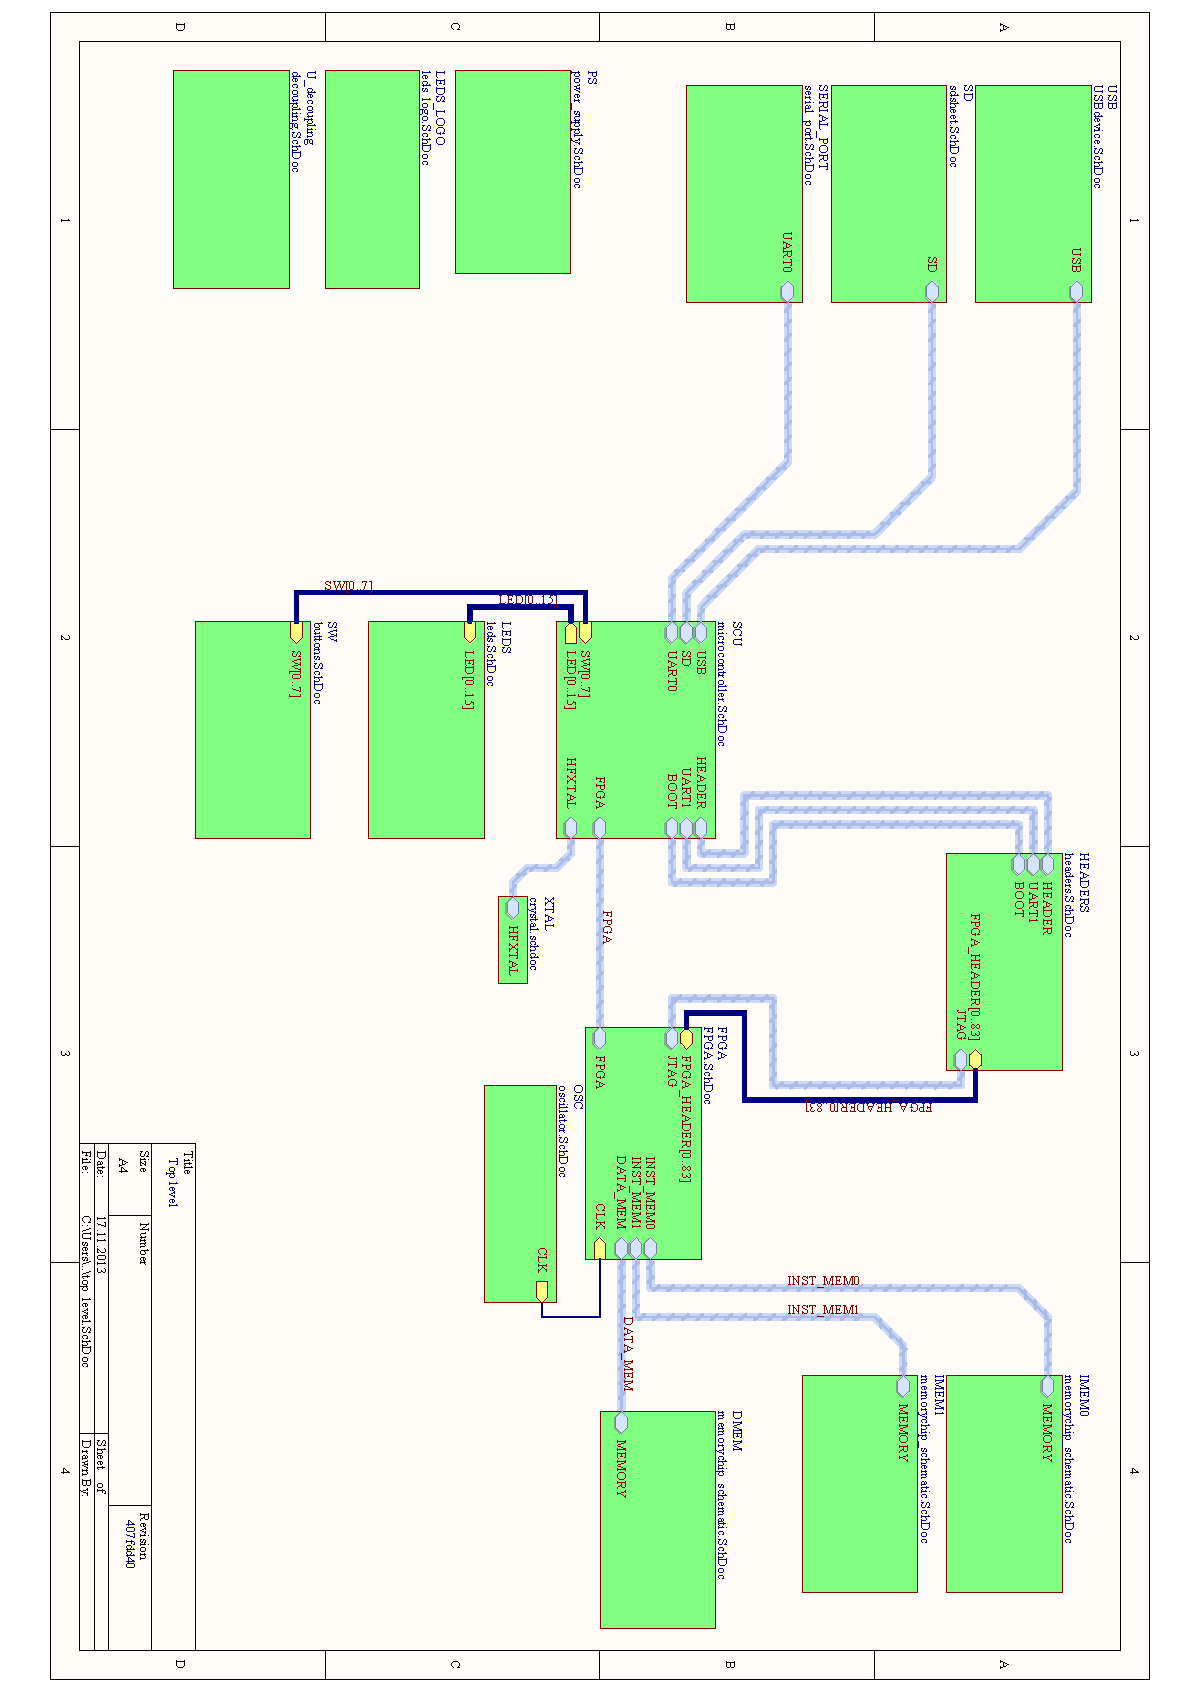
\includepdf[pages=-]{appendix/PCB_TDT4295_NTNU_2013_rotated.16.pdf}
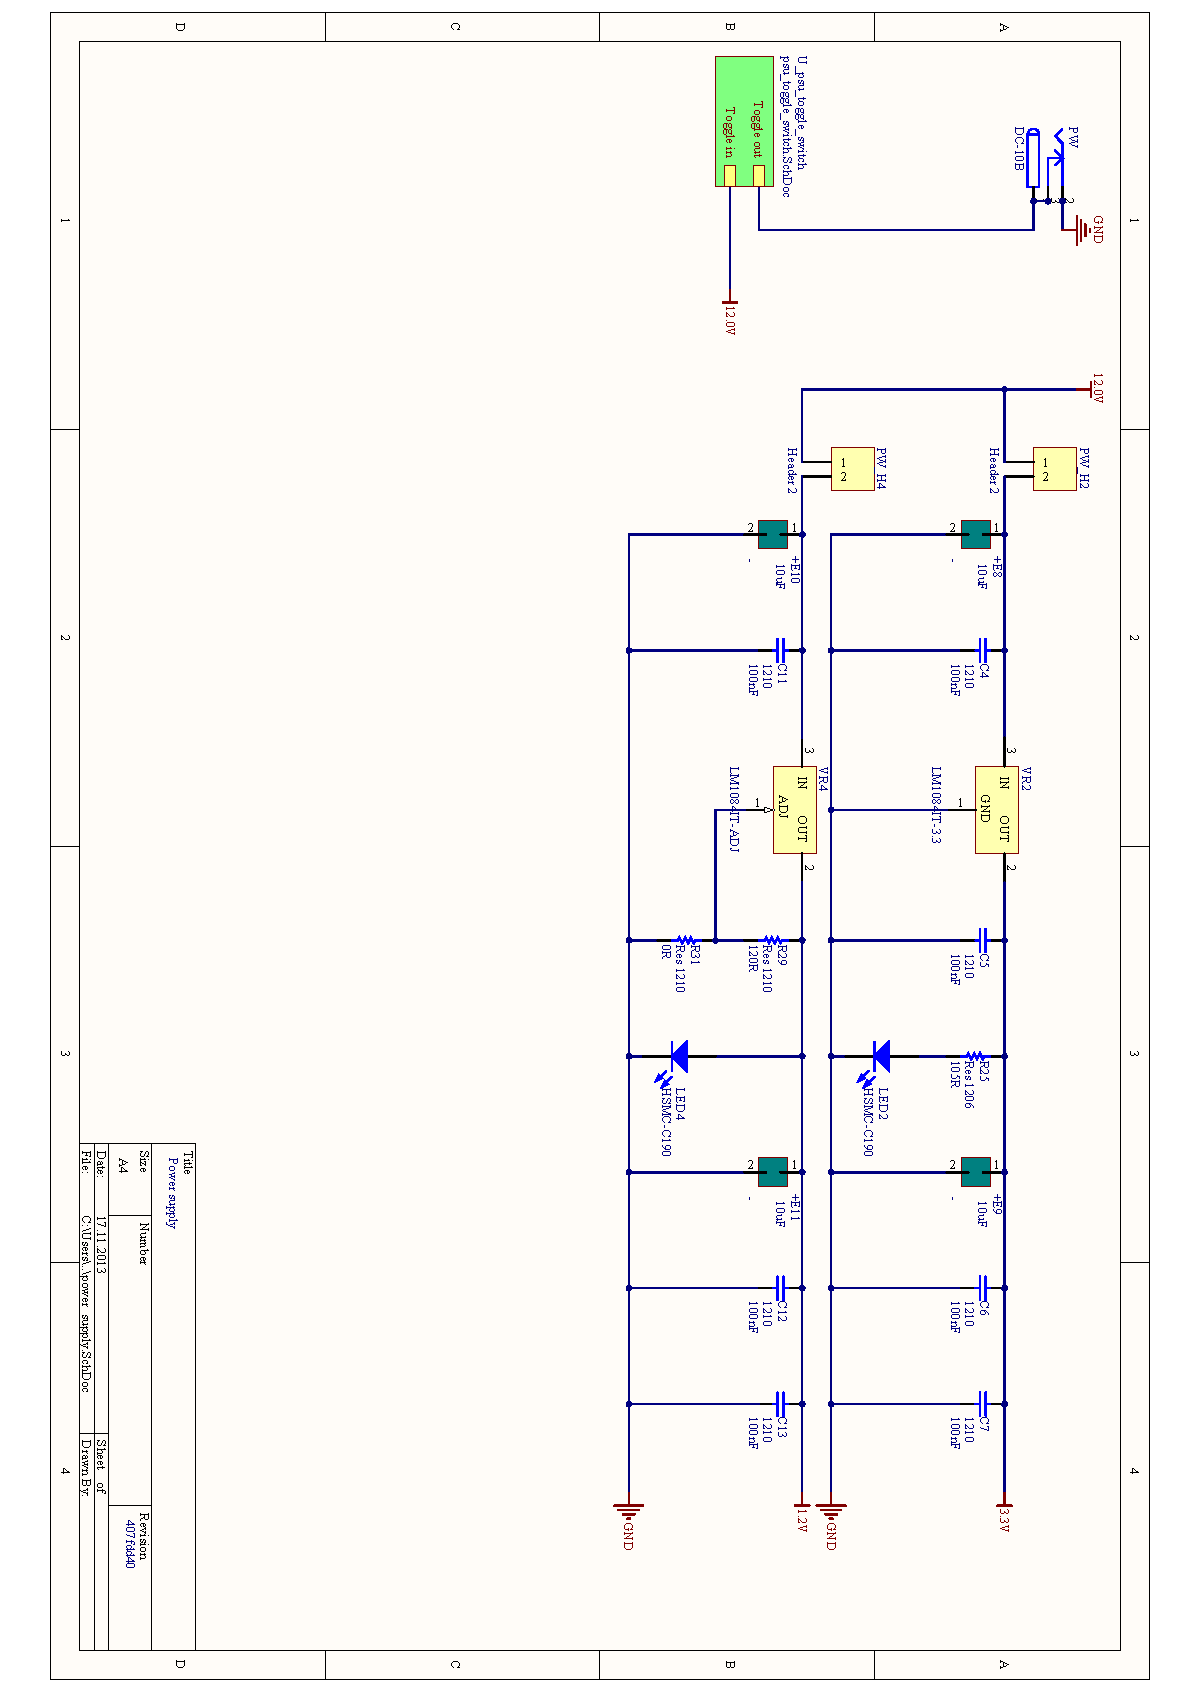
\includepdf[pages=-]{appendix/PCB_TDT4295_NTNU_2013_rotated.12.pdf}
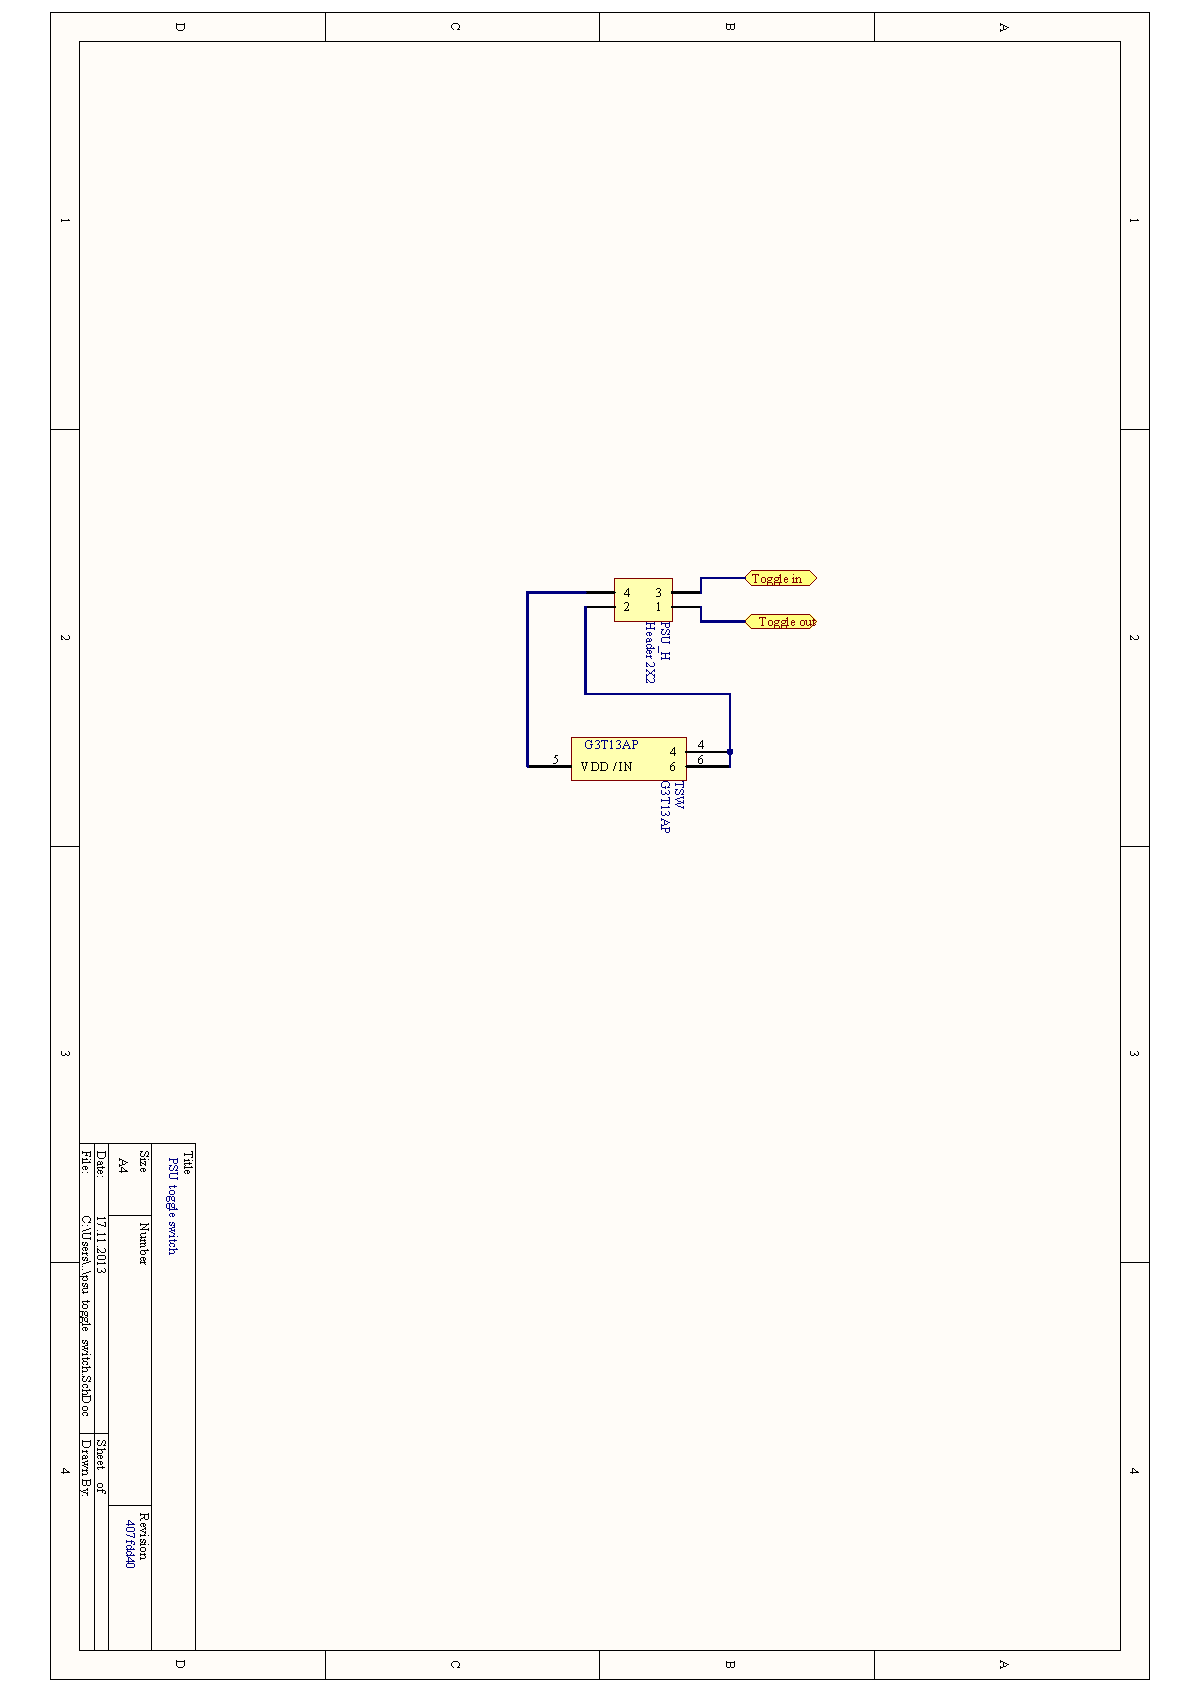
\includepdf[pages=-]{appendix/PCB_TDT4295_NTNU_2013_rotated.13.pdf}
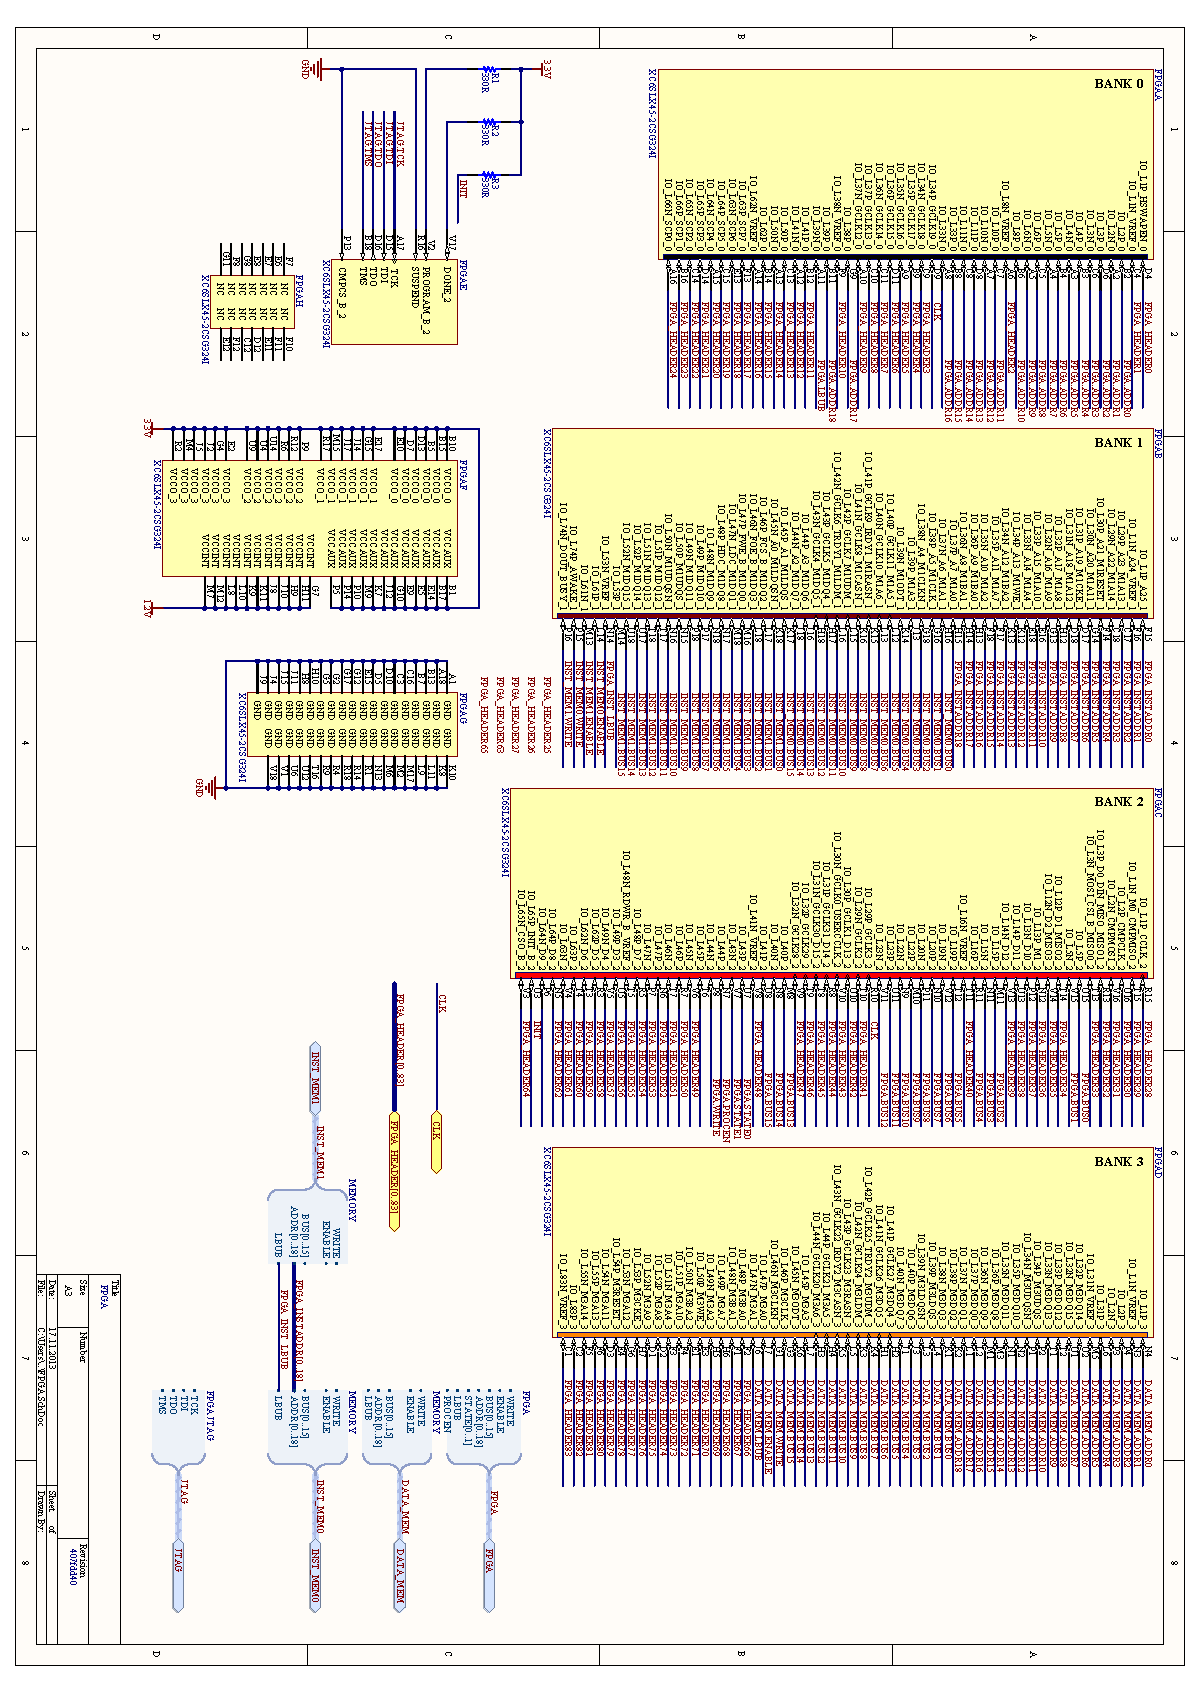
\includepdf[pages=-]{appendix/PCB_TDT4295_NTNU_2013_rotated.4.pdf}
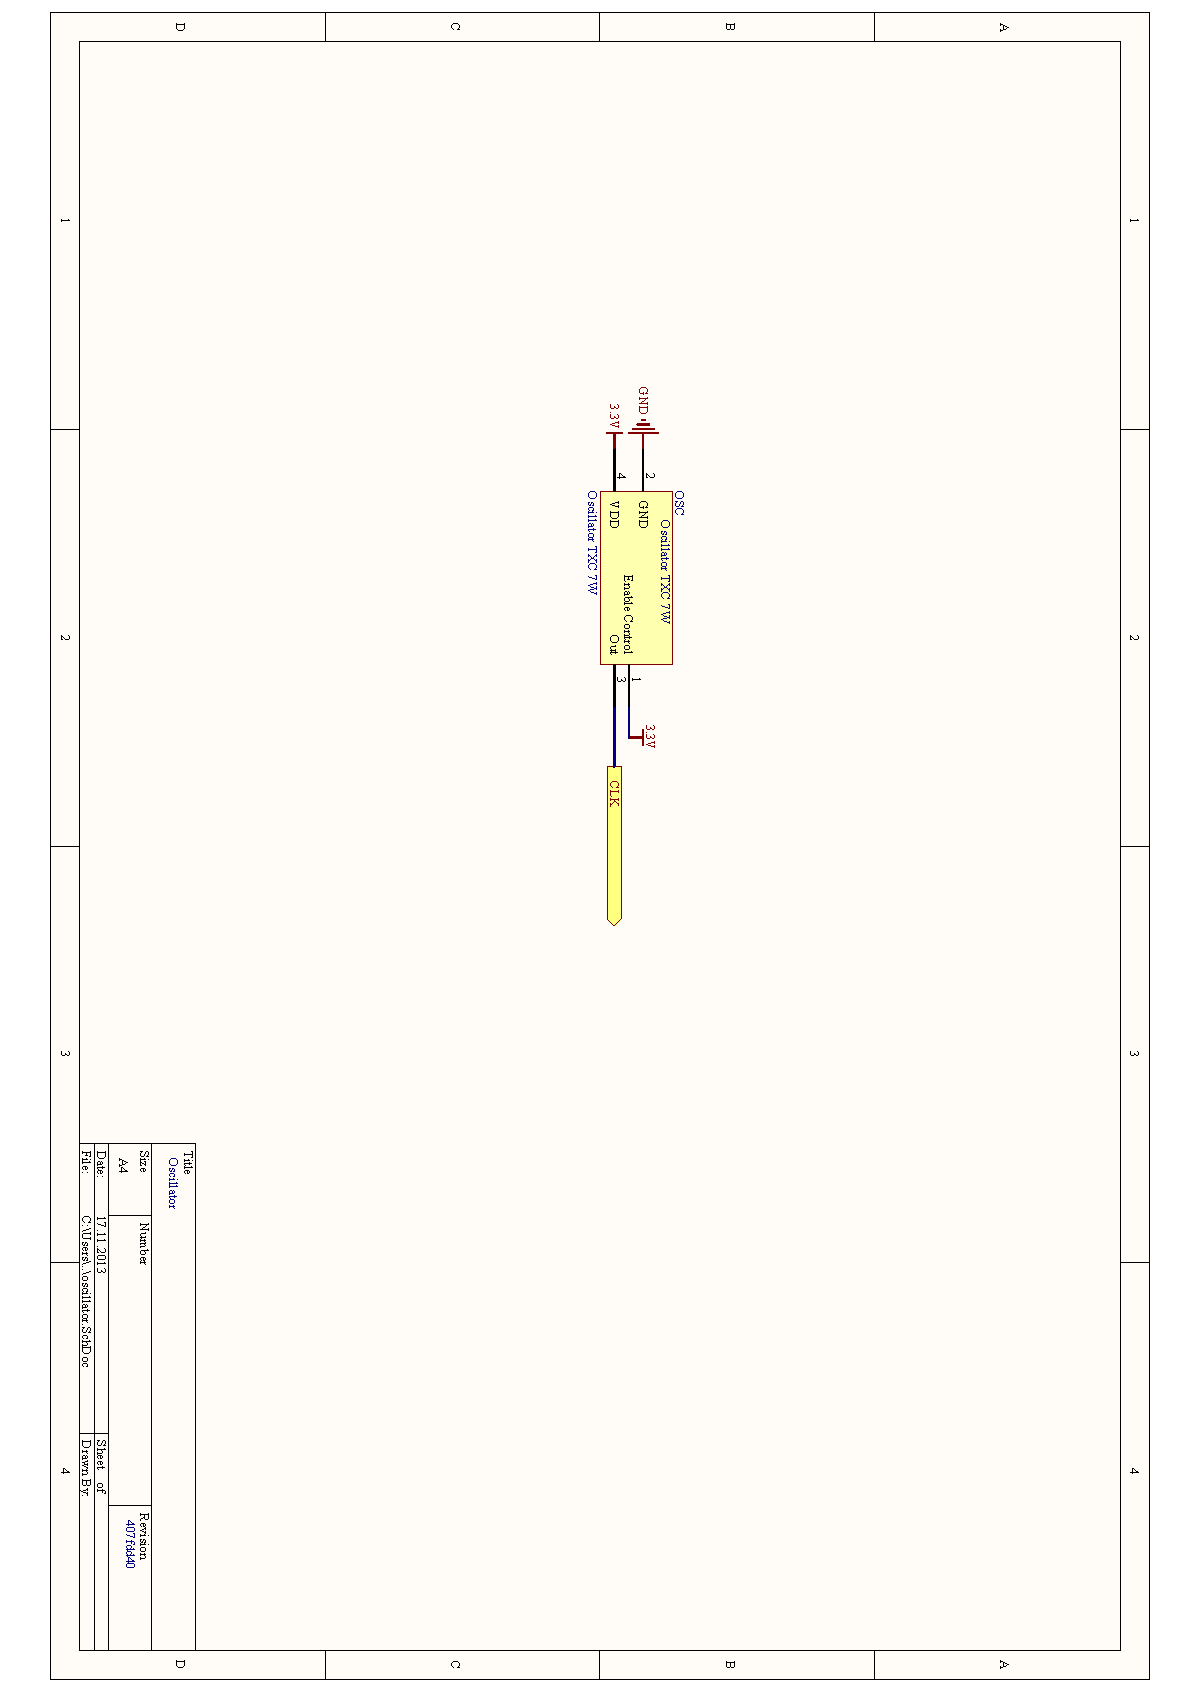
\includepdf[pages=-]{appendix/PCB_TDT4295_NTNU_2013_rotated.11.pdf}
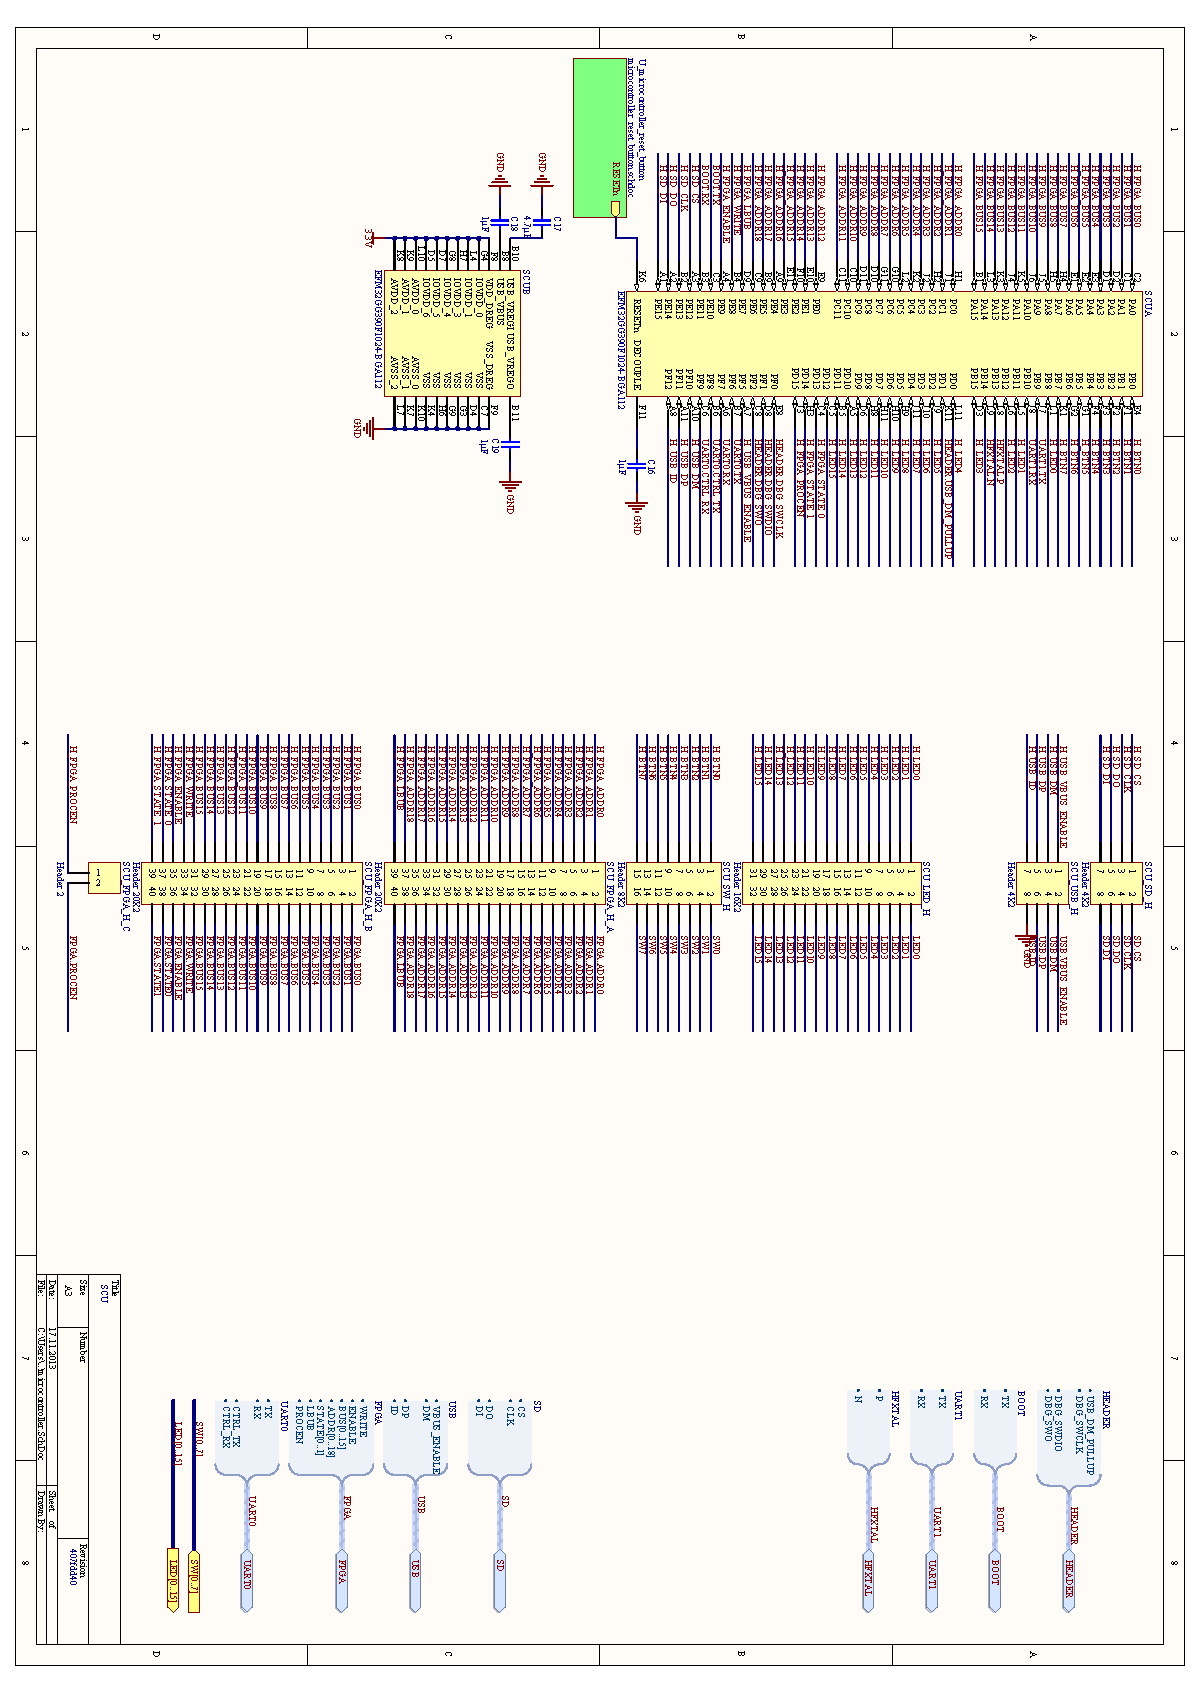
\includepdf[pages=-]{appendix/PCB_TDT4295_NTNU_2013_rotated.9.pdf}
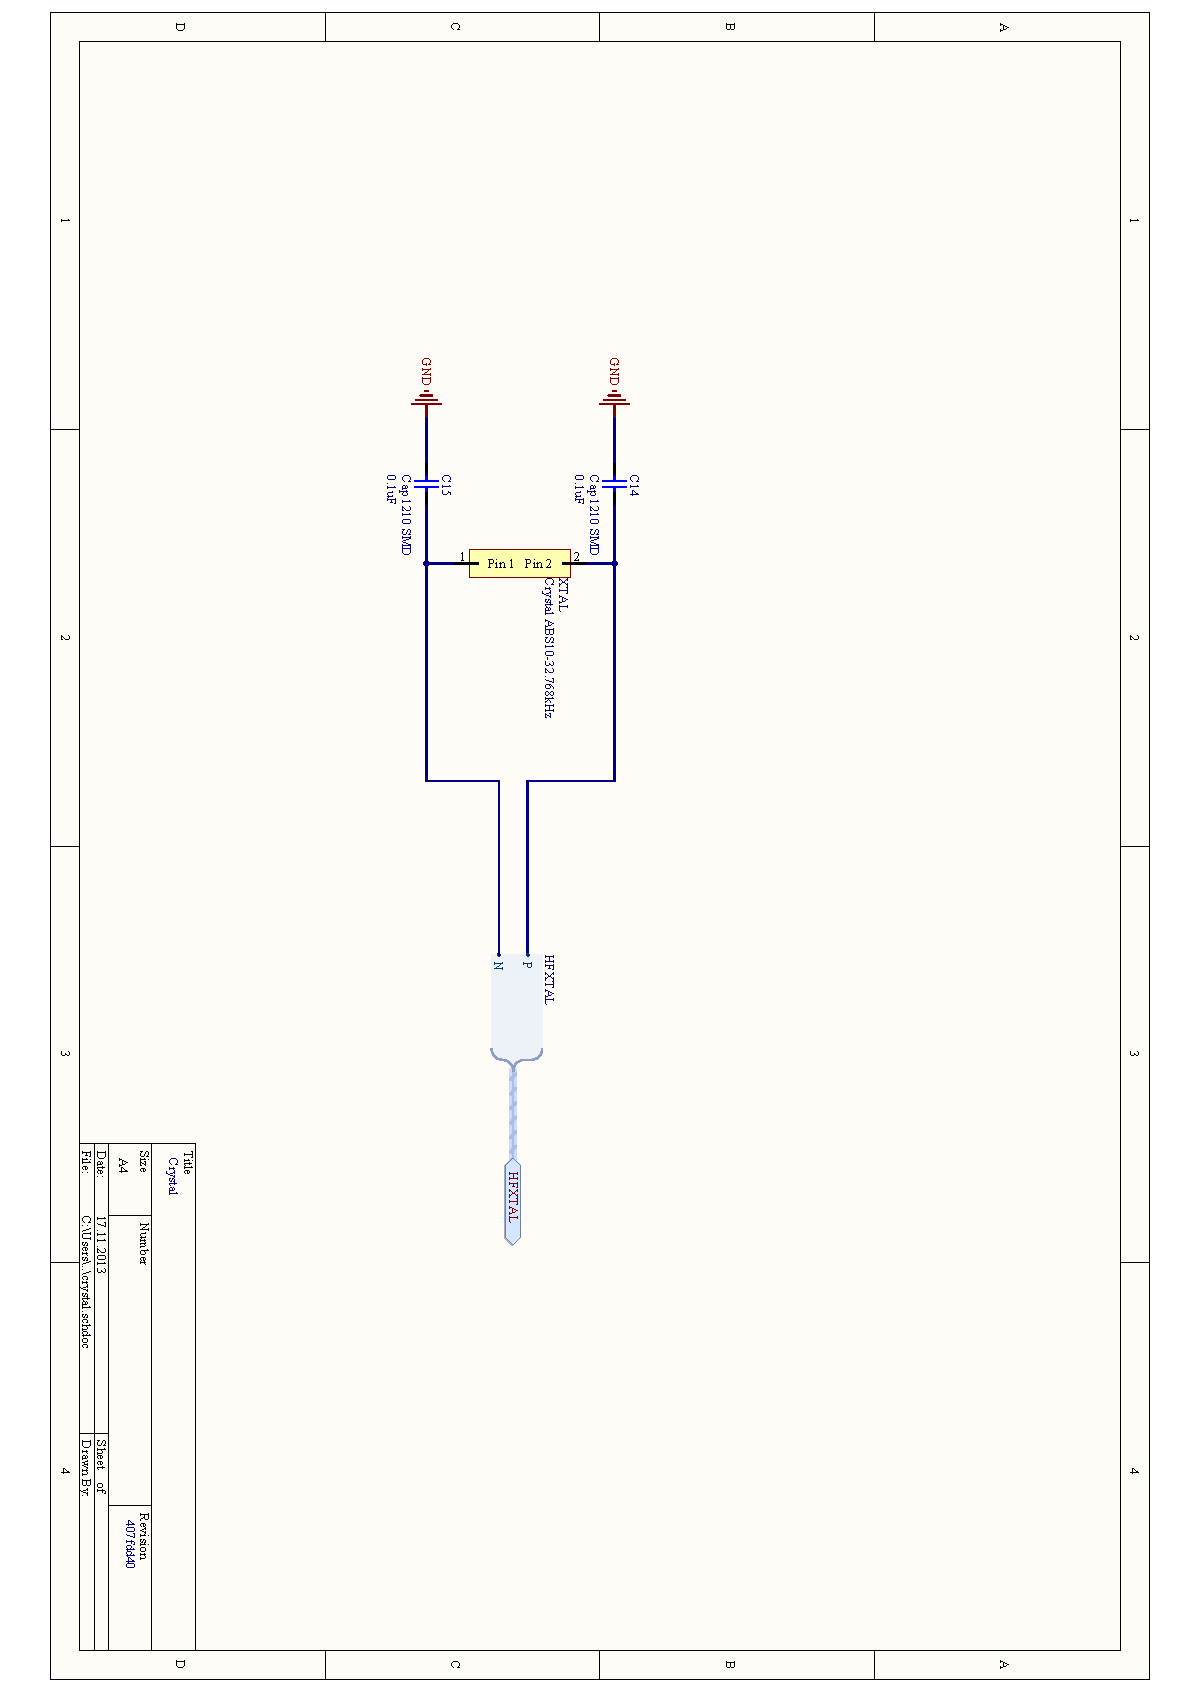
\includepdf[pages=-]{appendix/PCB_TDT4295_NTNU_2013_rotated.2.pdf}
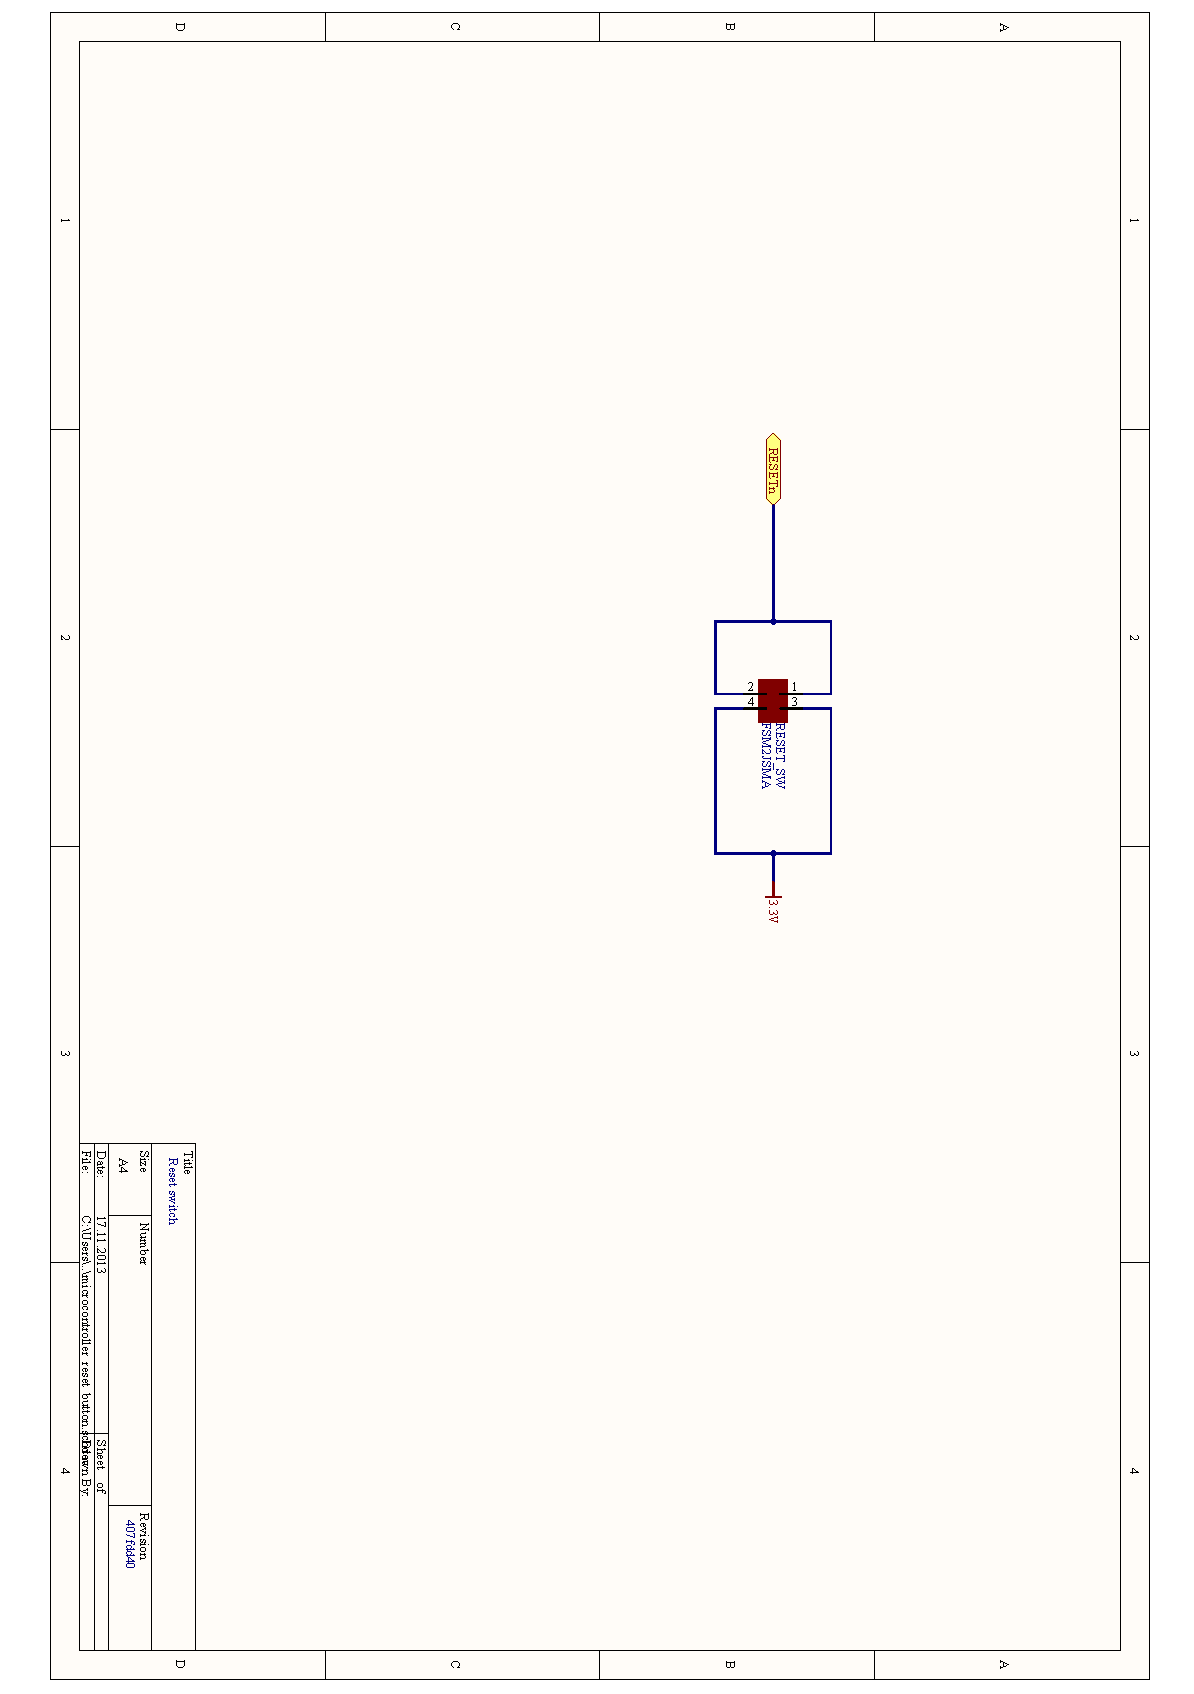
\includepdf[pages=-]{appendix/PCB_TDT4295_NTNU_2013_rotated.10.pdf}
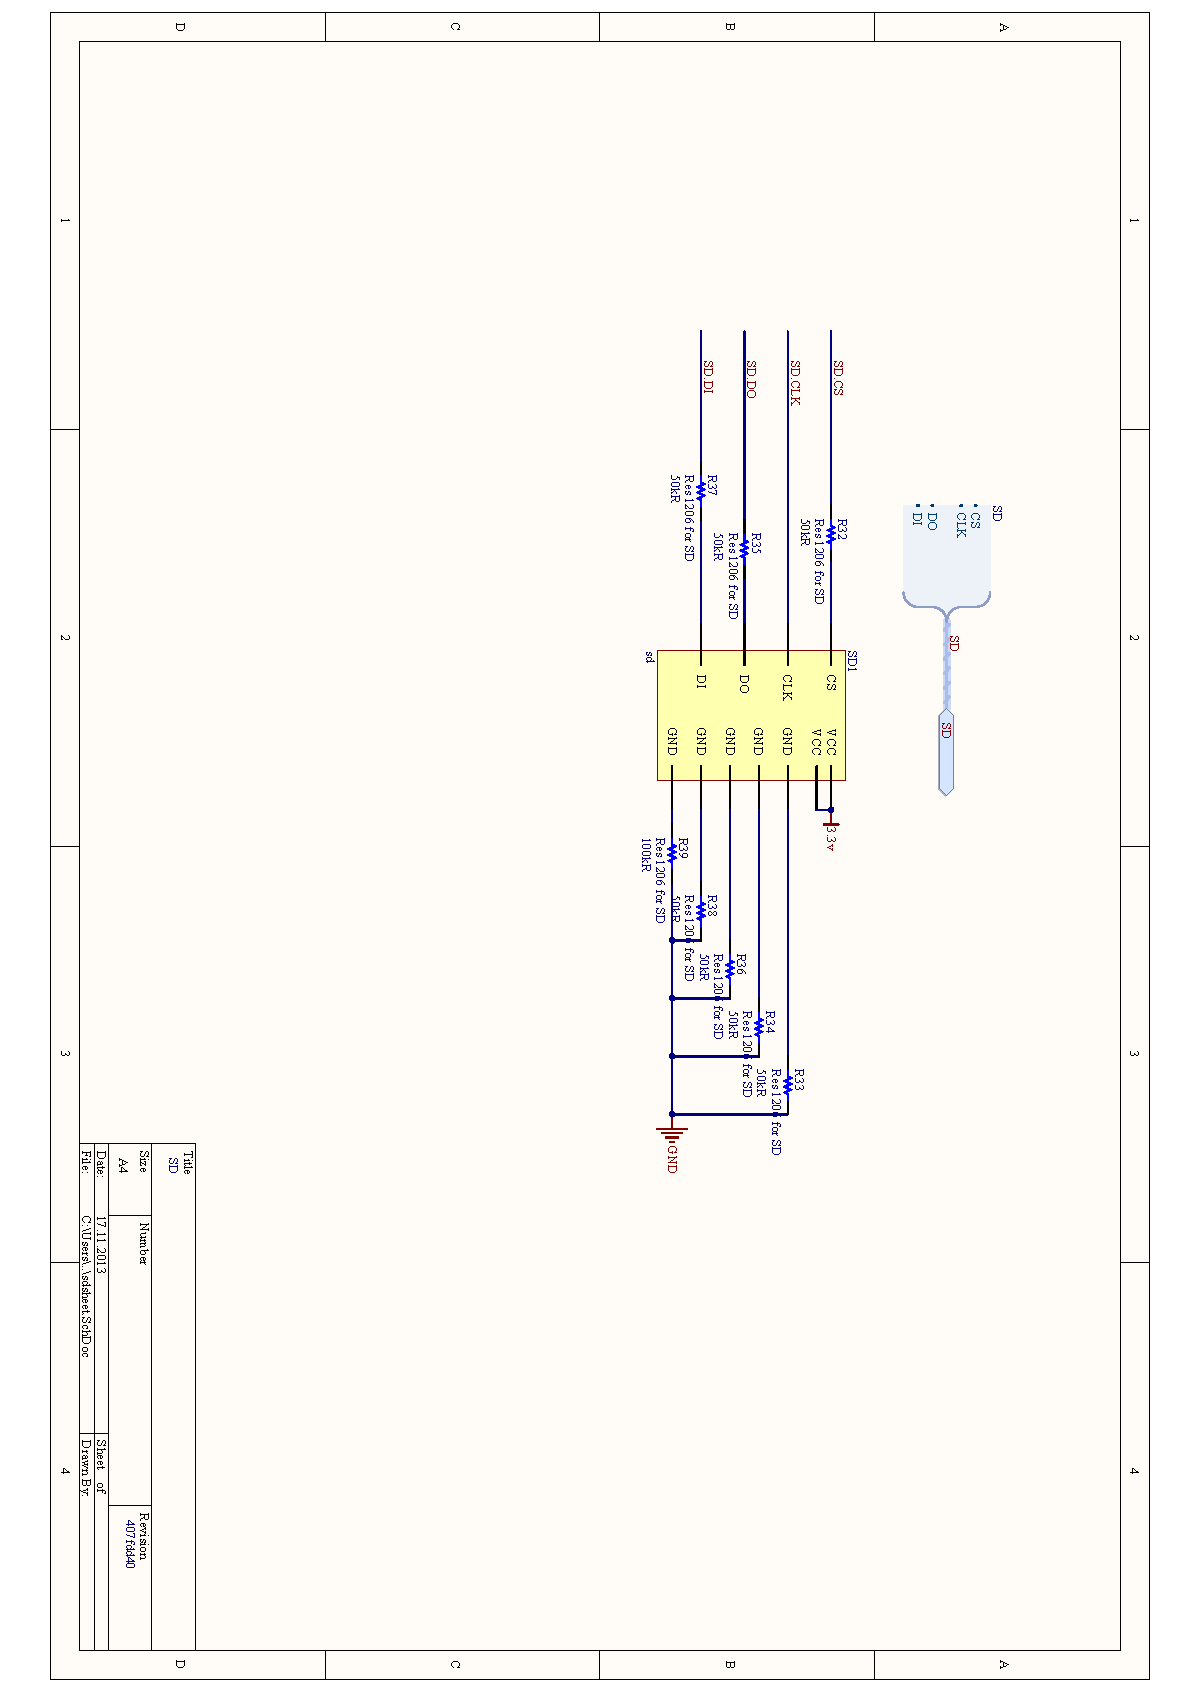
\includepdf[pages=-]{appendix/PCB_TDT4295_NTNU_2013_rotated.14.pdf}
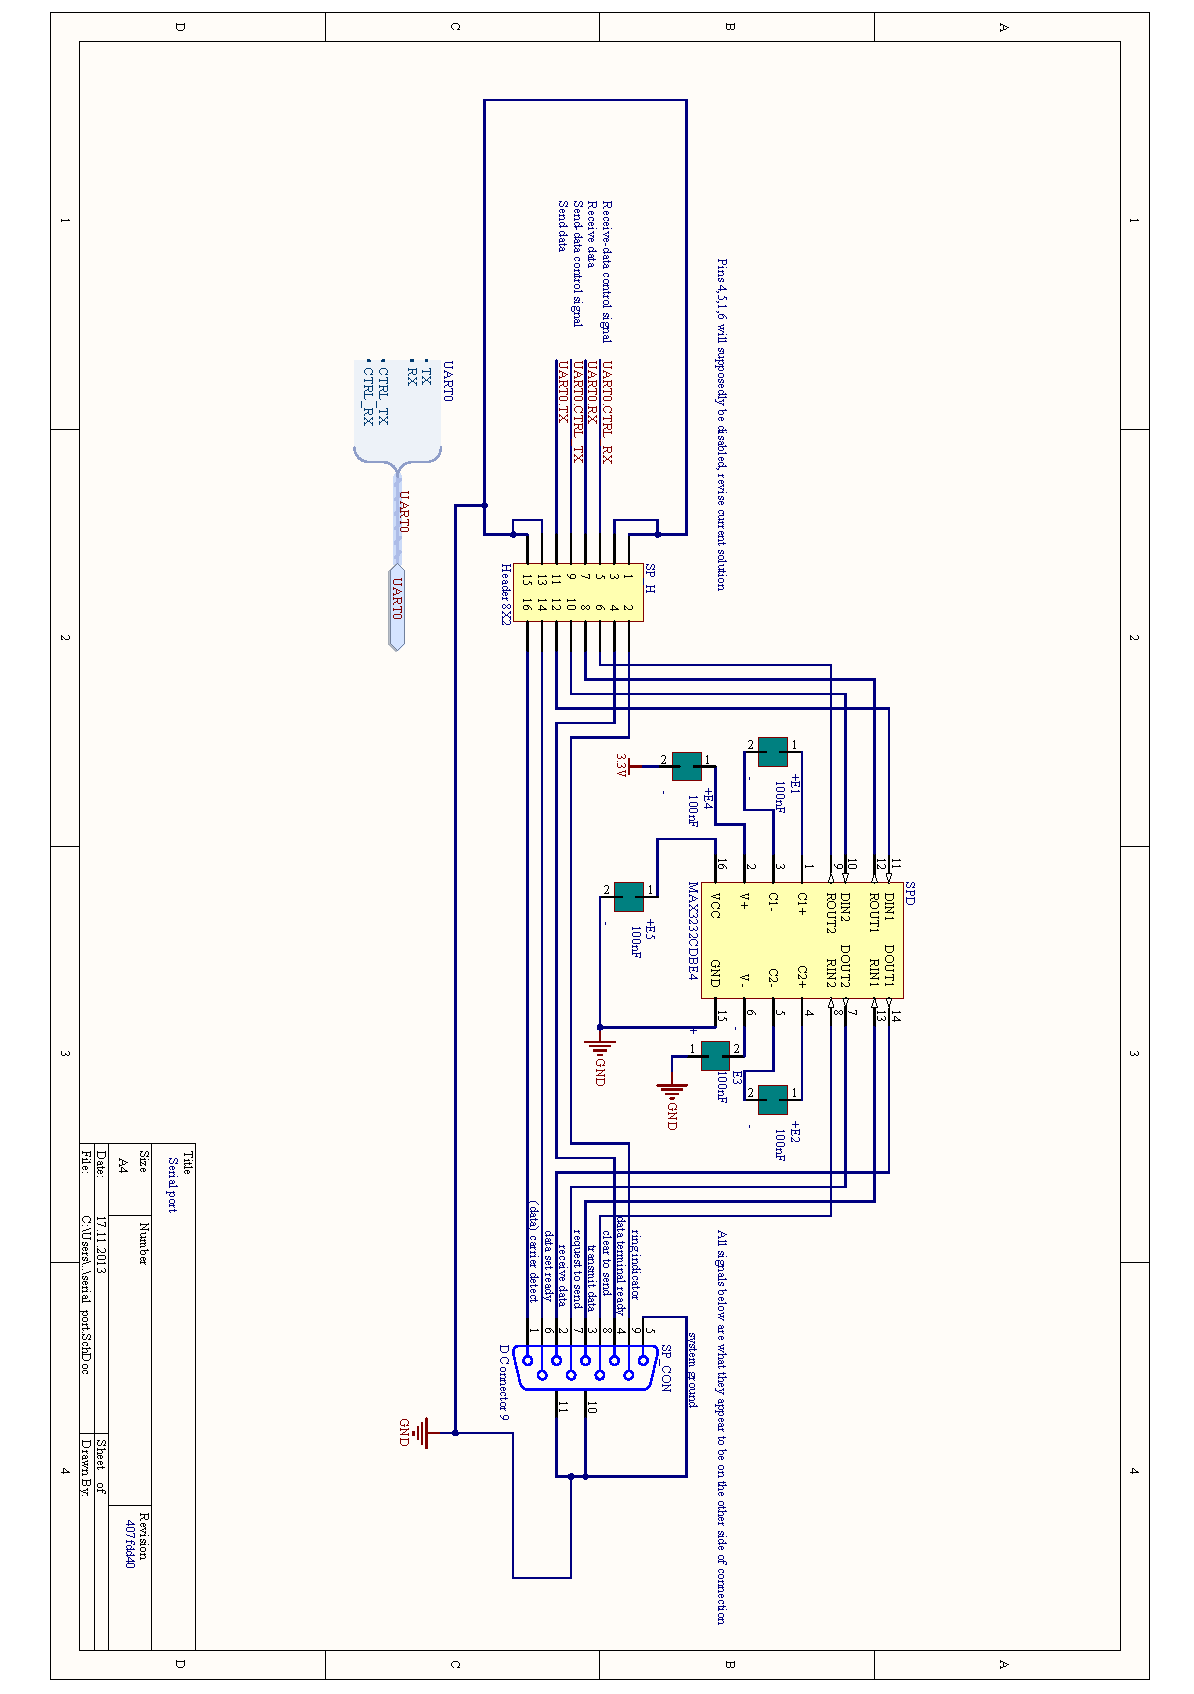
\includepdf[pages=-]{appendix/PCB_TDT4295_NTNU_2013_rotated.15.pdf}
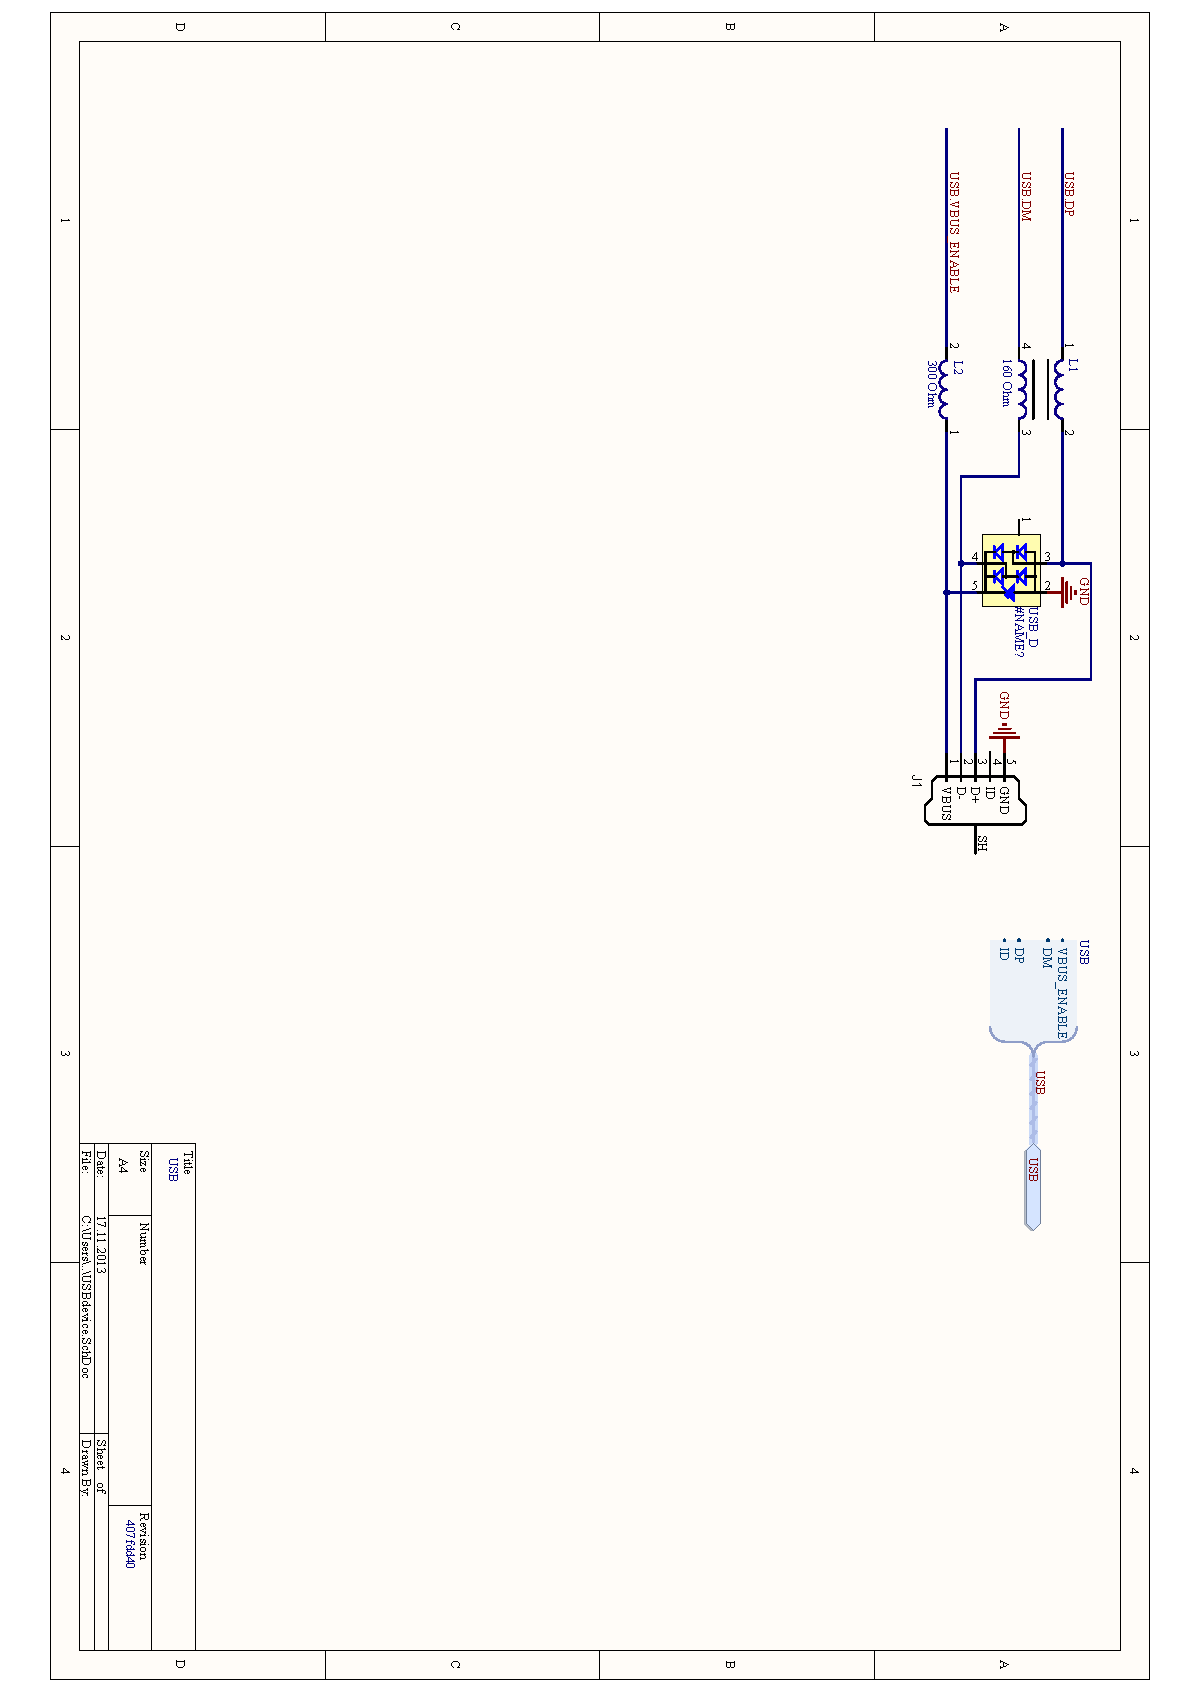
\includepdf[pages=-]{appendix/PCB_TDT4295_NTNU_2013_rotated.17.pdf}
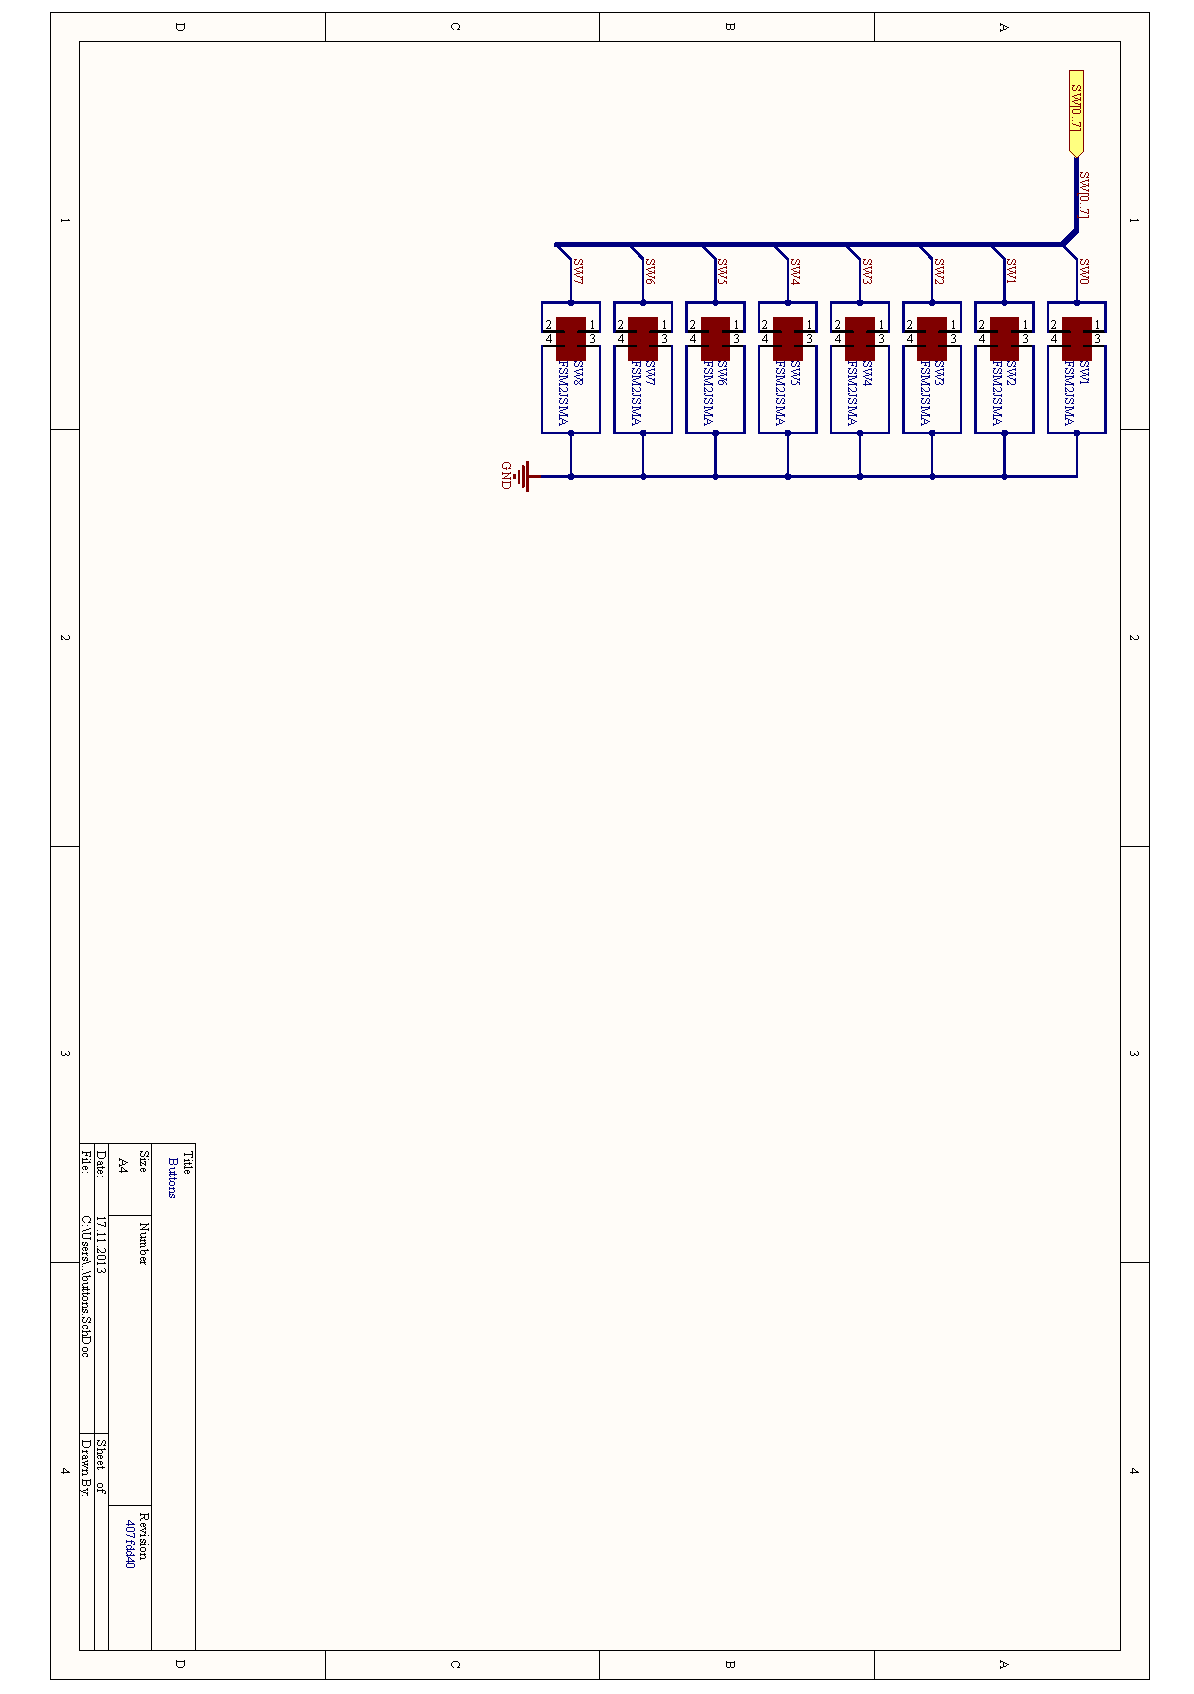
\includepdf[pages=-]{appendix/PCB_TDT4295_NTNU_2013_rotated.1.pdf}
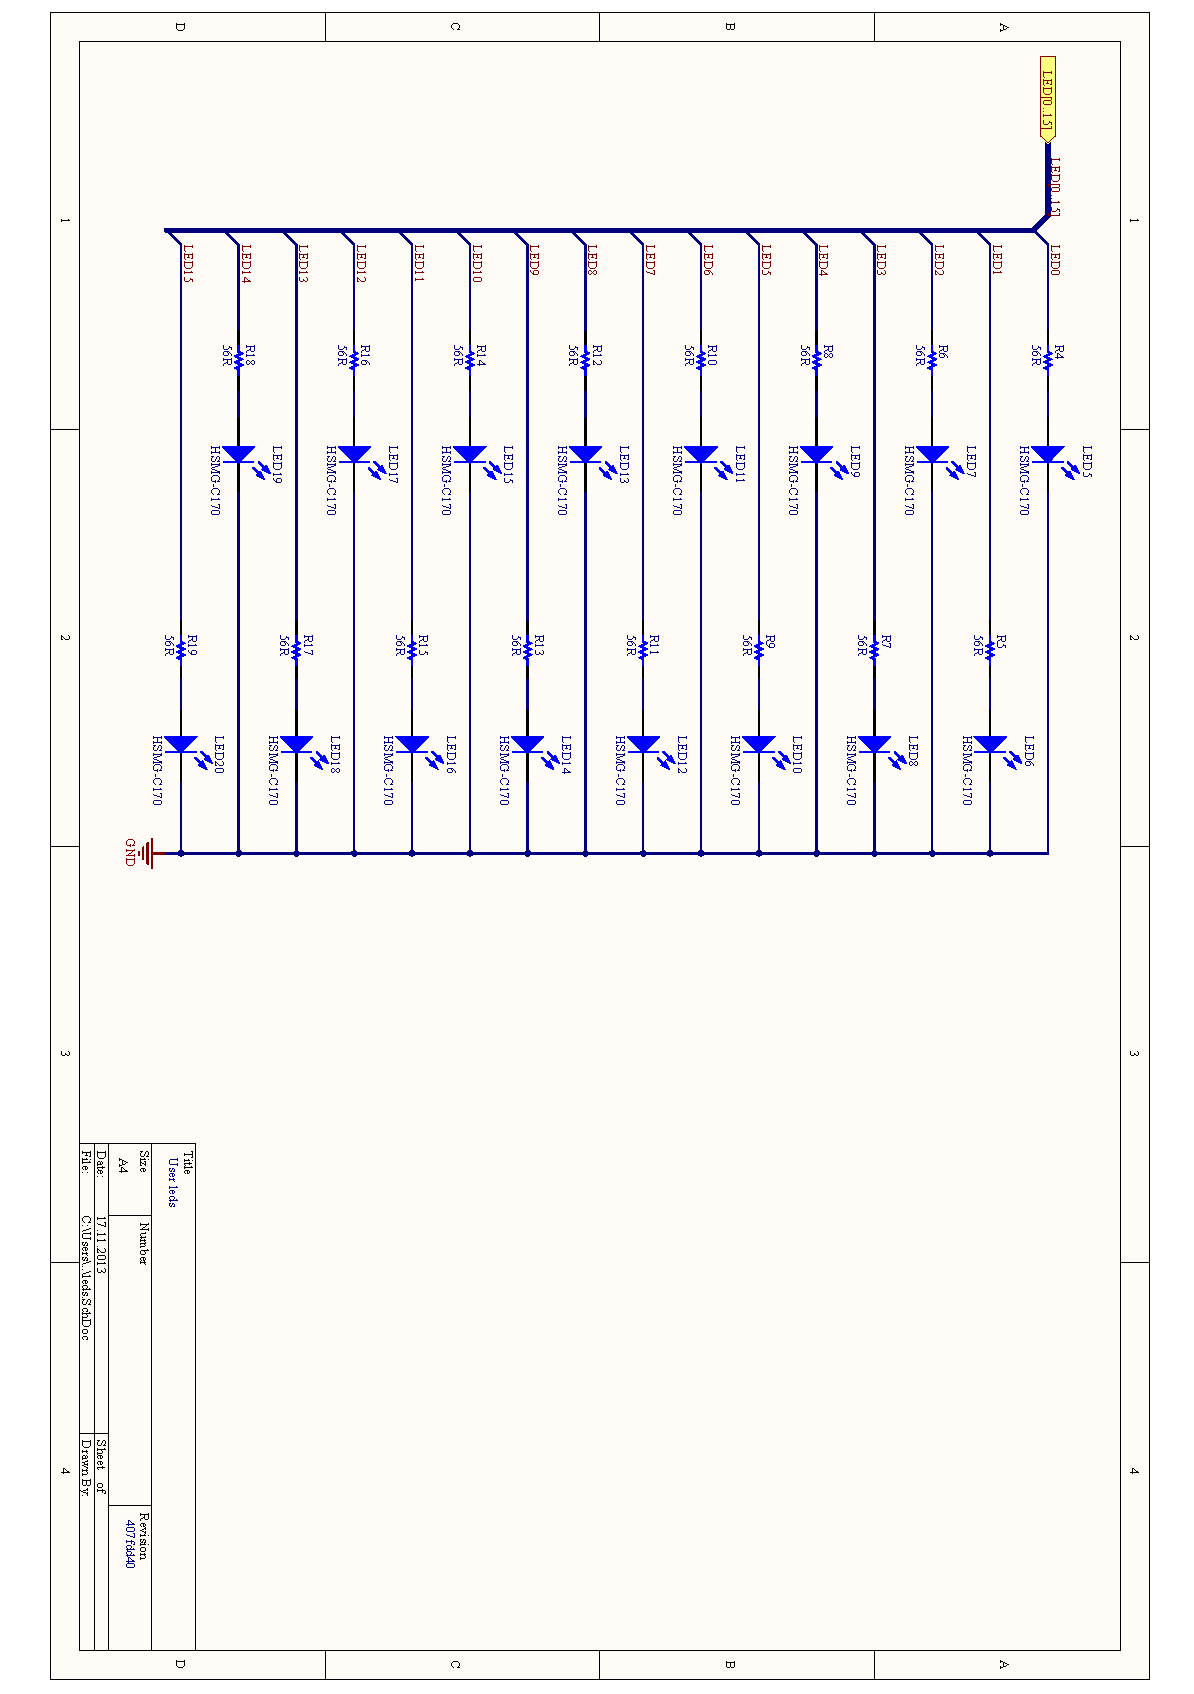
\includepdf[pages=-]{appendix/PCB_TDT4295_NTNU_2013_rotated.6.pdf}
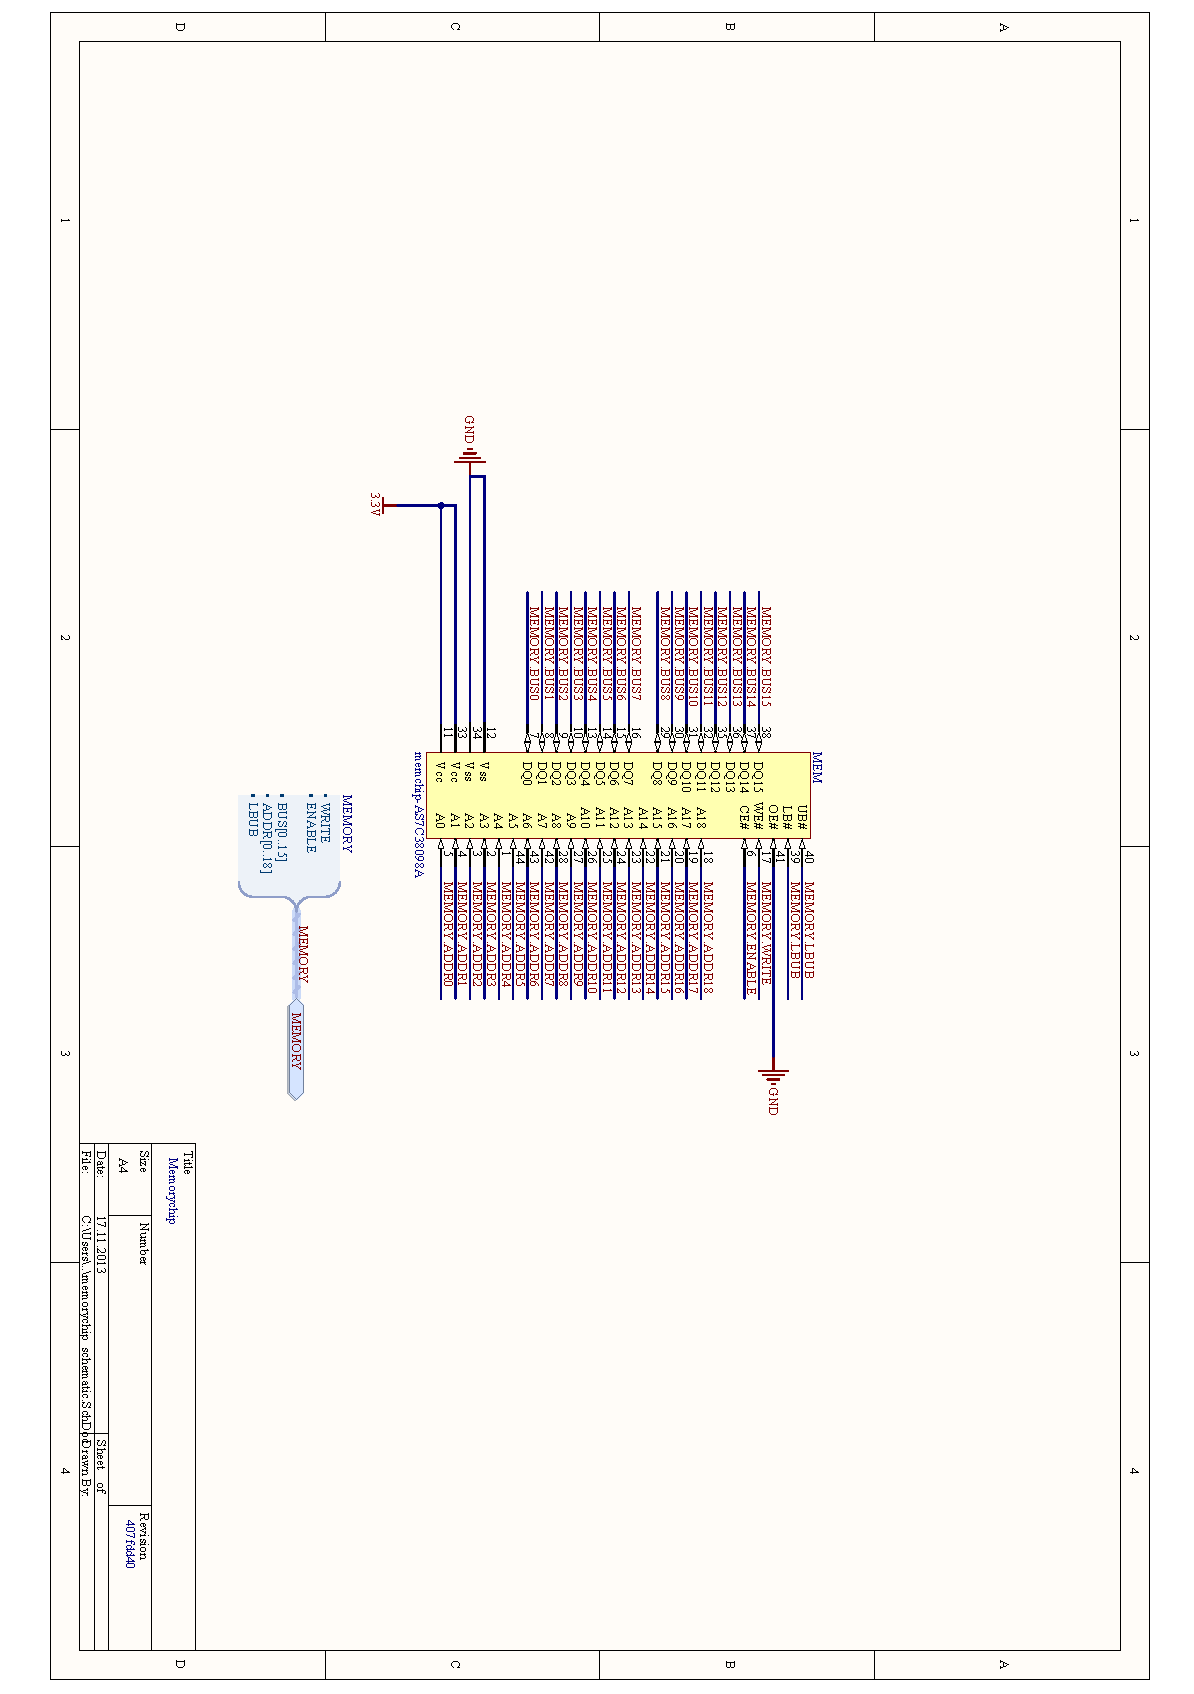
\includepdf[pages=-]{appendix/PCB_TDT4295_NTNU_2013_rotated.8.pdf}
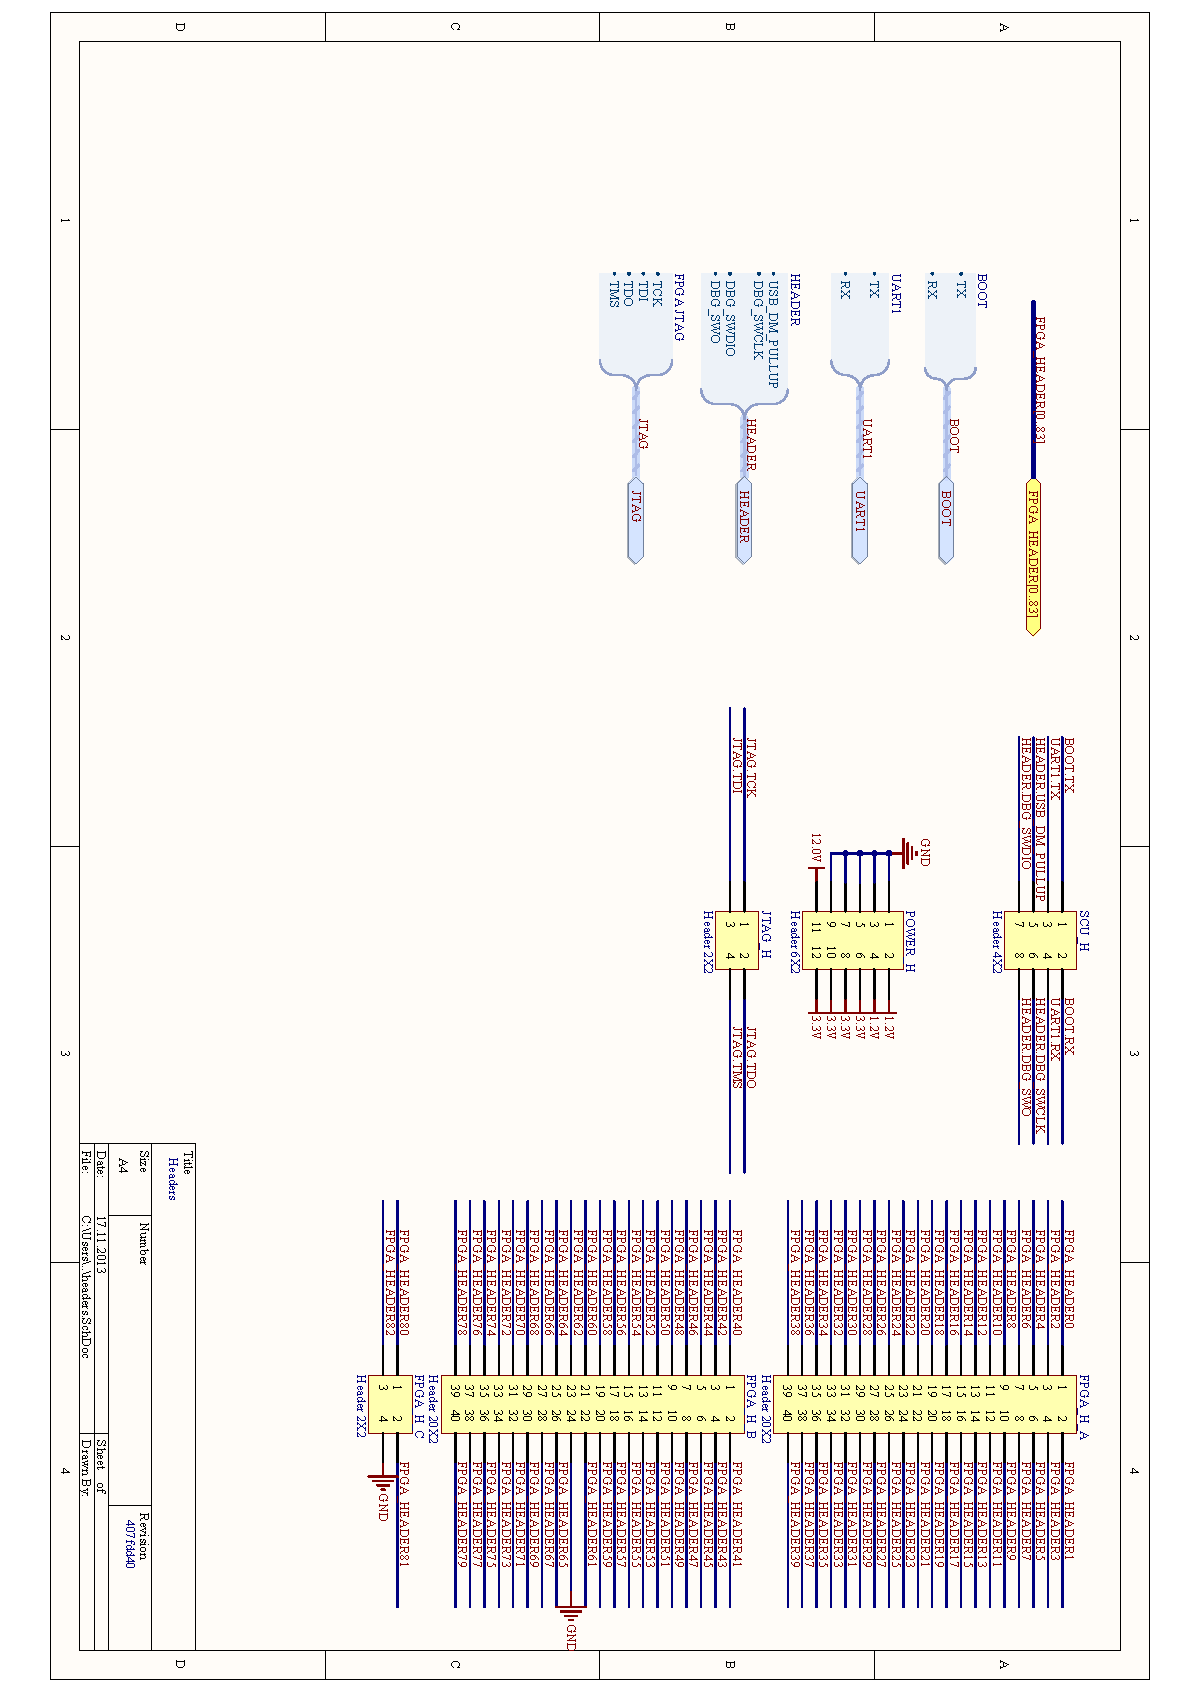
\includepdf[pages=-]{appendix/PCB_TDT4295_NTNU_2013_rotated.5.pdf}
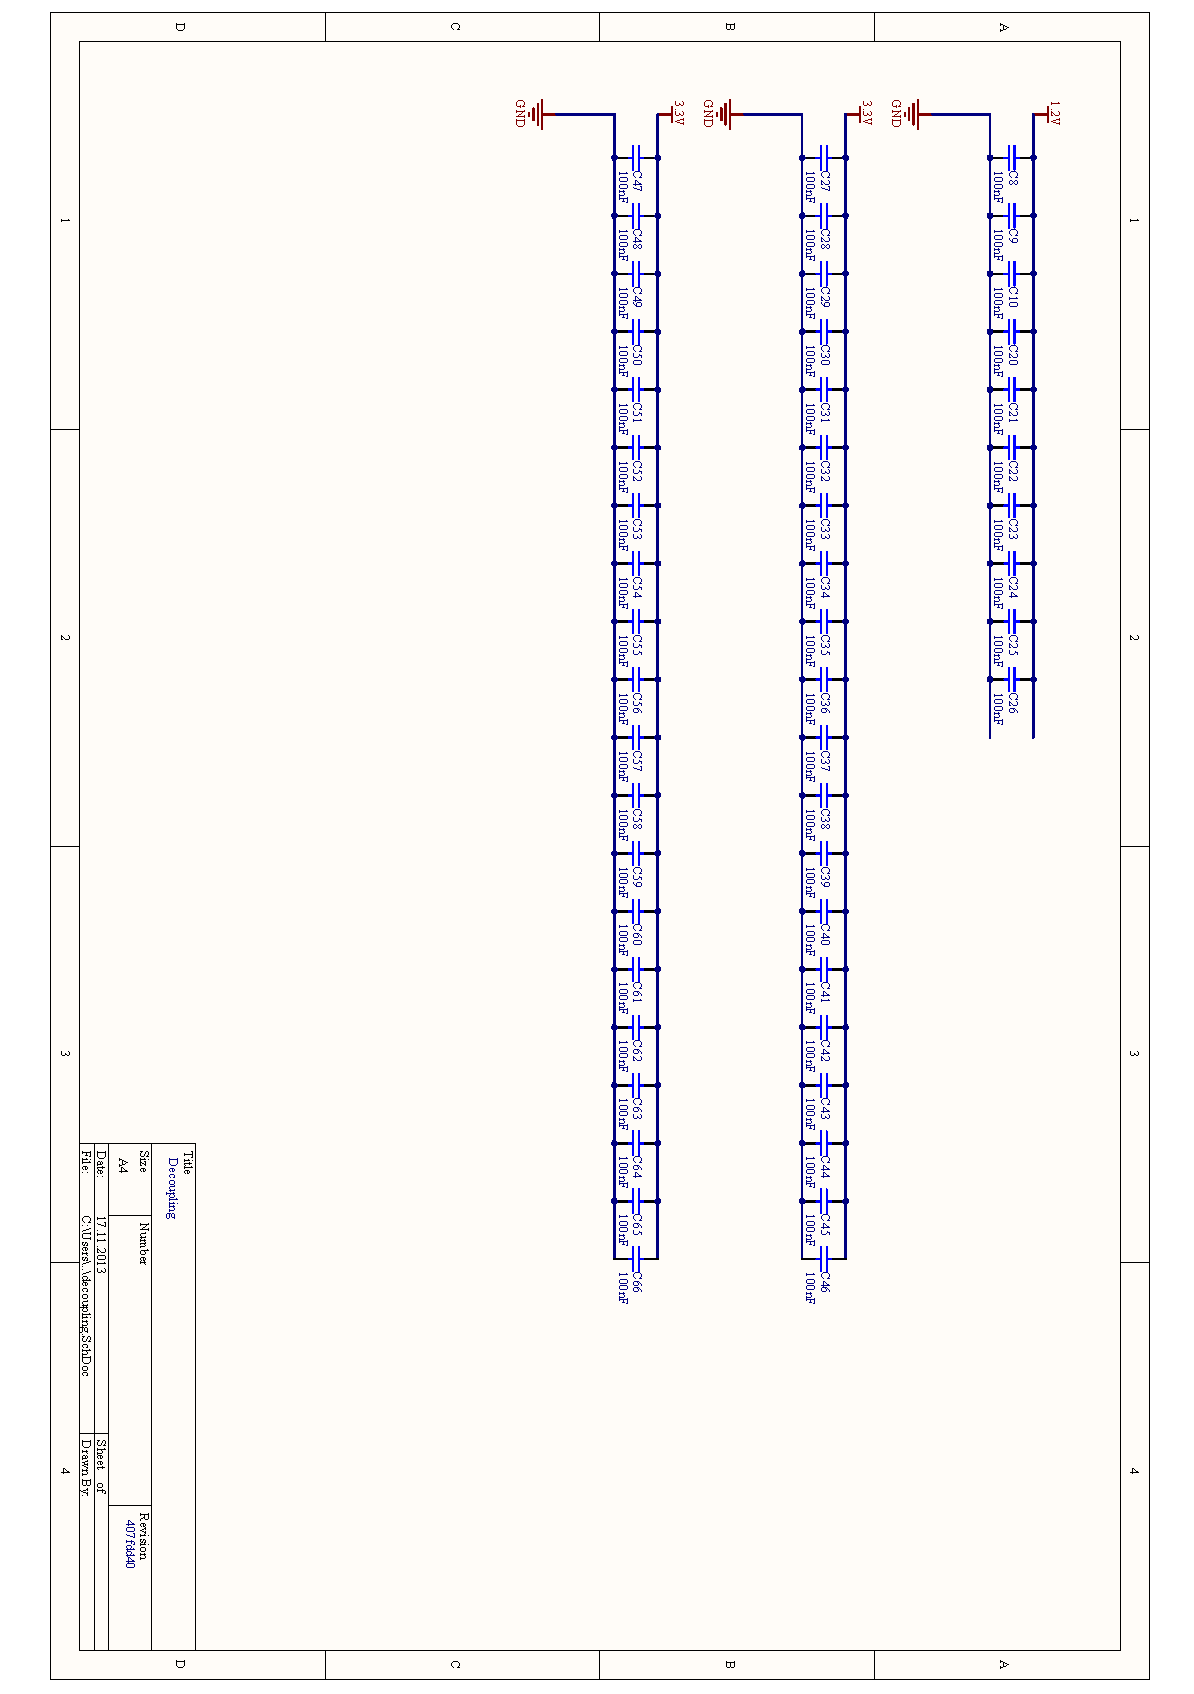
\includepdf[pages=-]{appendix/PCB_TDT4295_NTNU_2013_rotated.3.pdf}
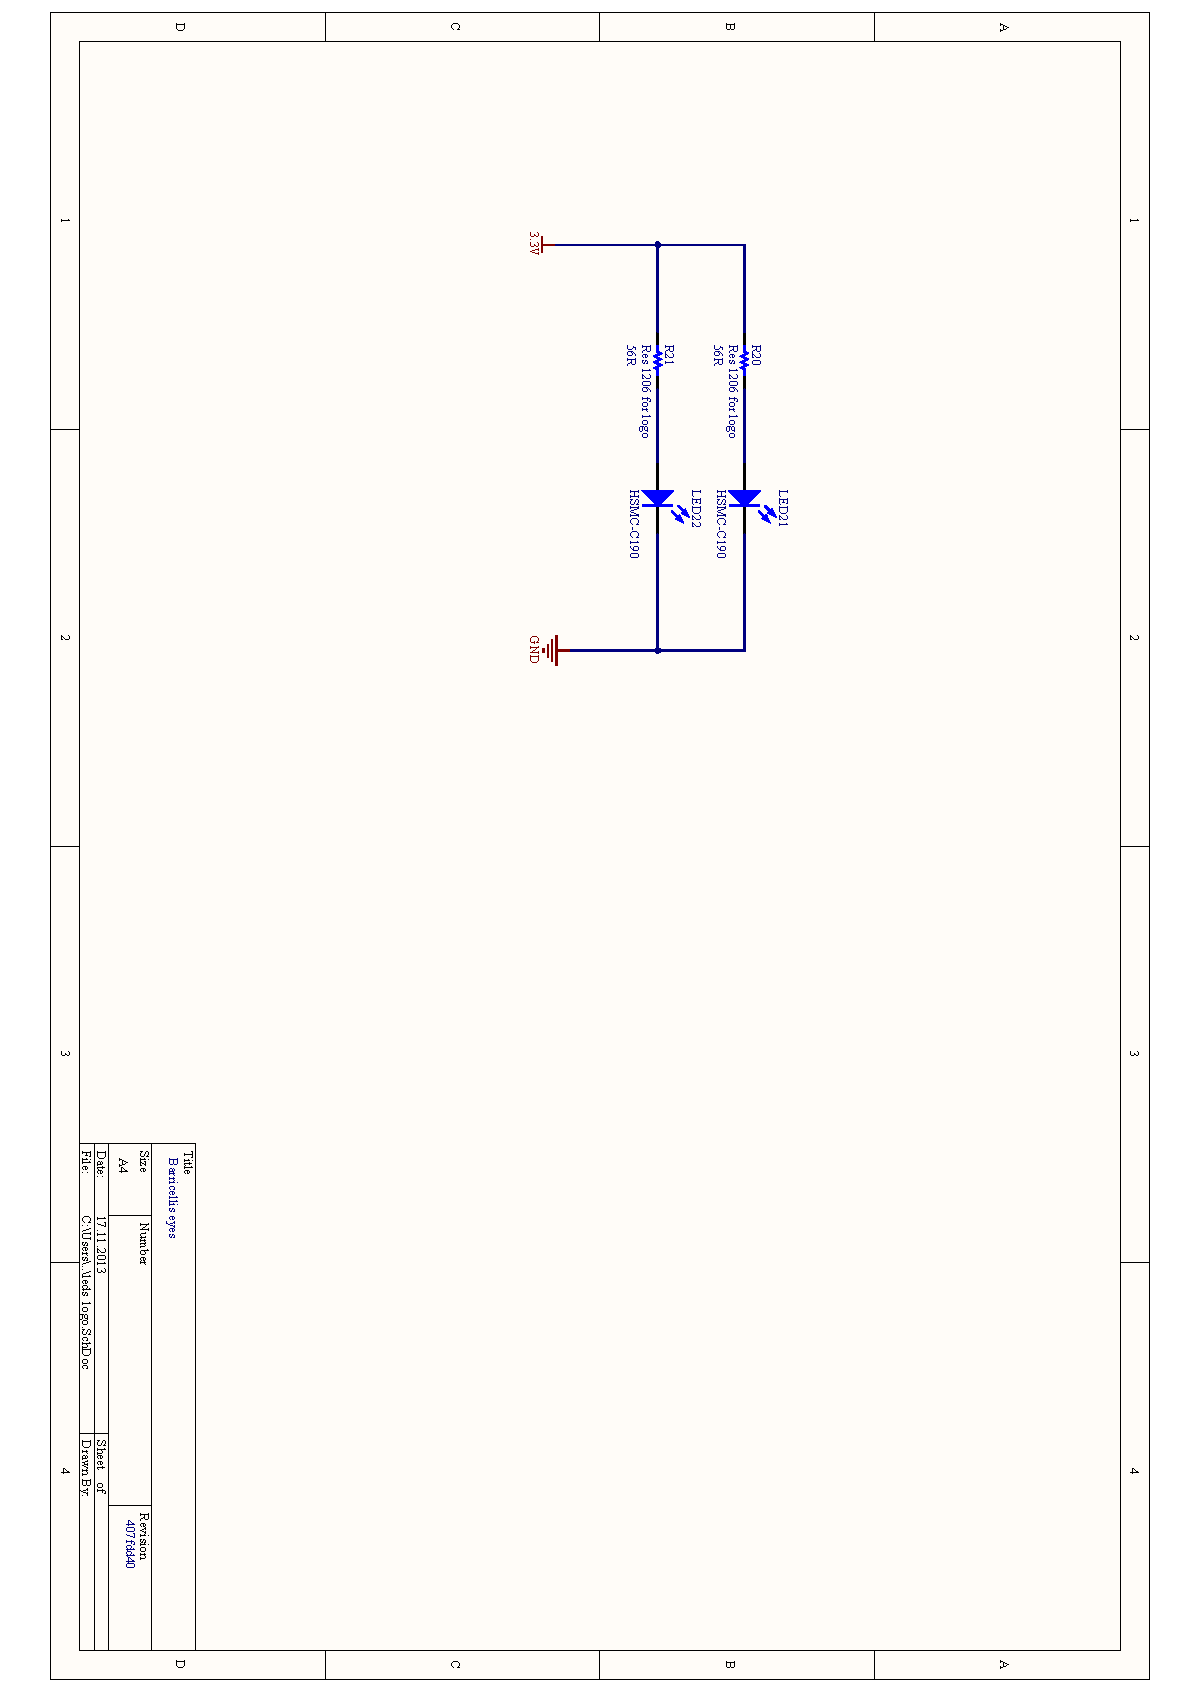
\includepdf[pages=-]{appendix/PCB_TDT4295_NTNU_2013_rotated.7.pdf}
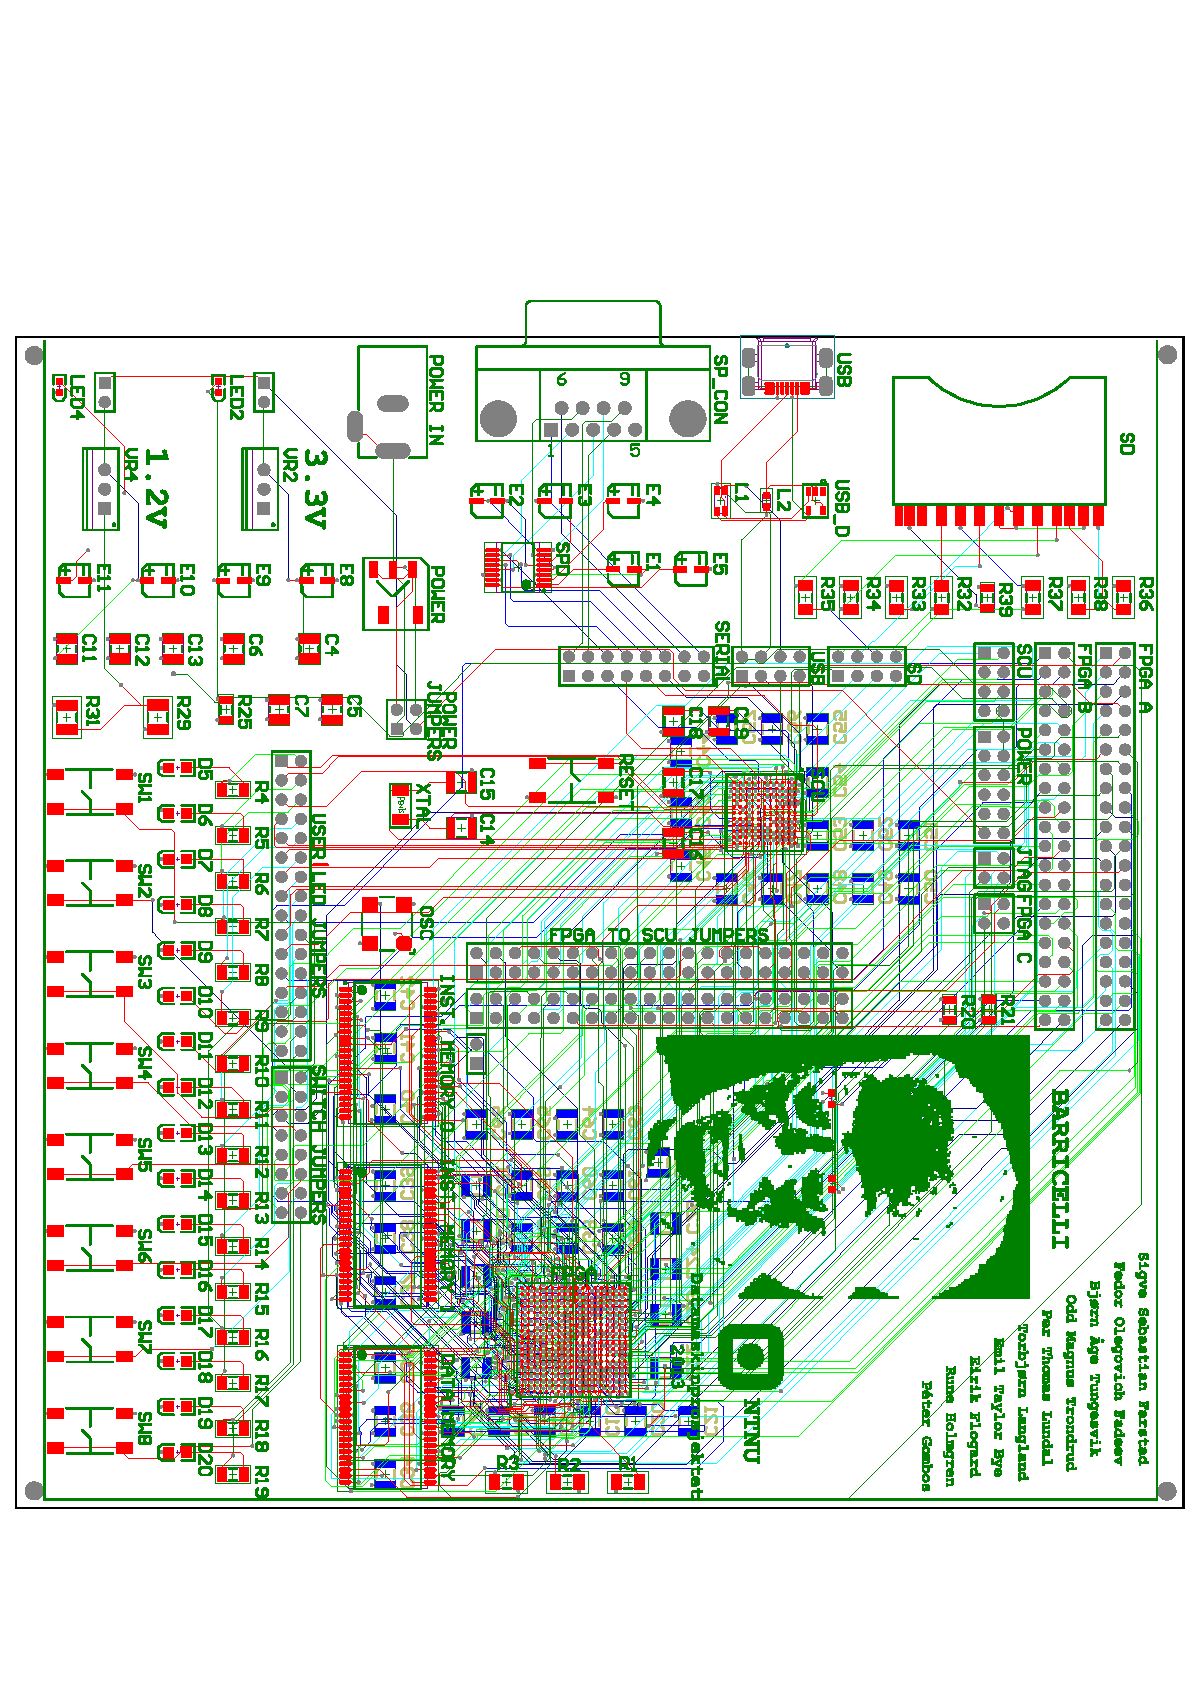
\includepdf[pages=-]{appendix/PCB_TDT4295_NTNU_2013_rotated.18.pdf}

\chapter{Case schematics} \label{appendix:case-schematics}
\newpage
\begin{figure}
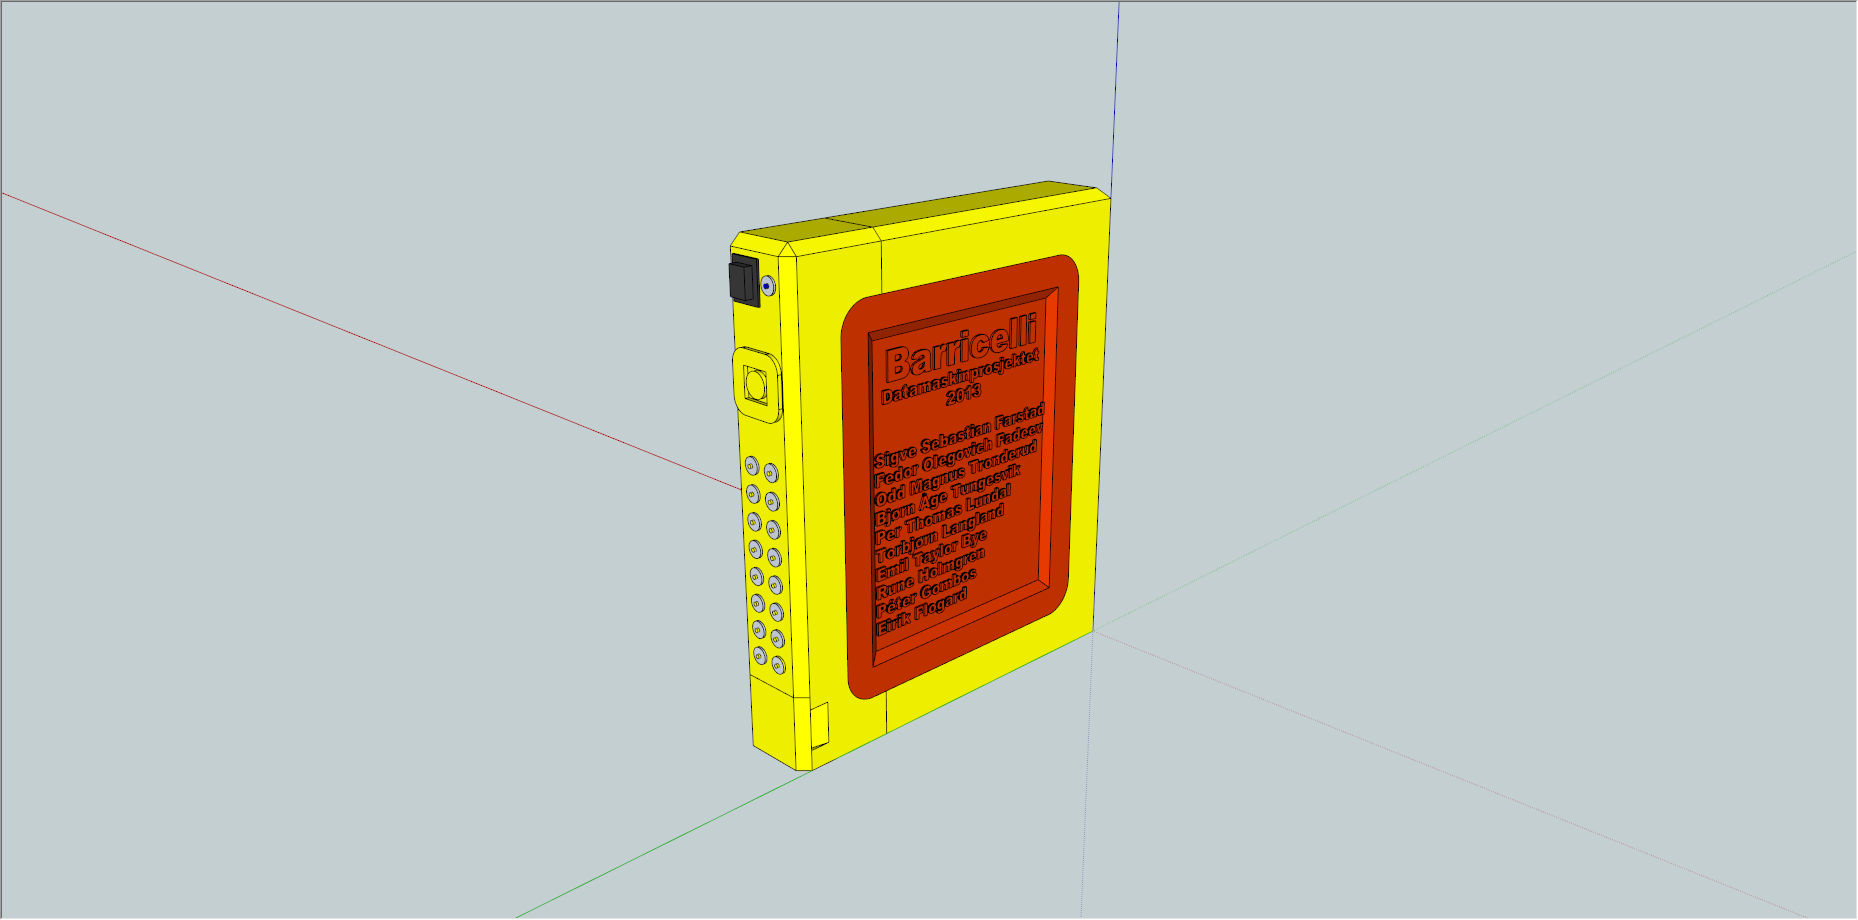
\includegraphics[width=\textwidth,keepaspectratio,clip]{appendix/screen-shots/outer-shell.png}%
\caption{Case design}
\end{figure}

\newpage
\begin{figure}
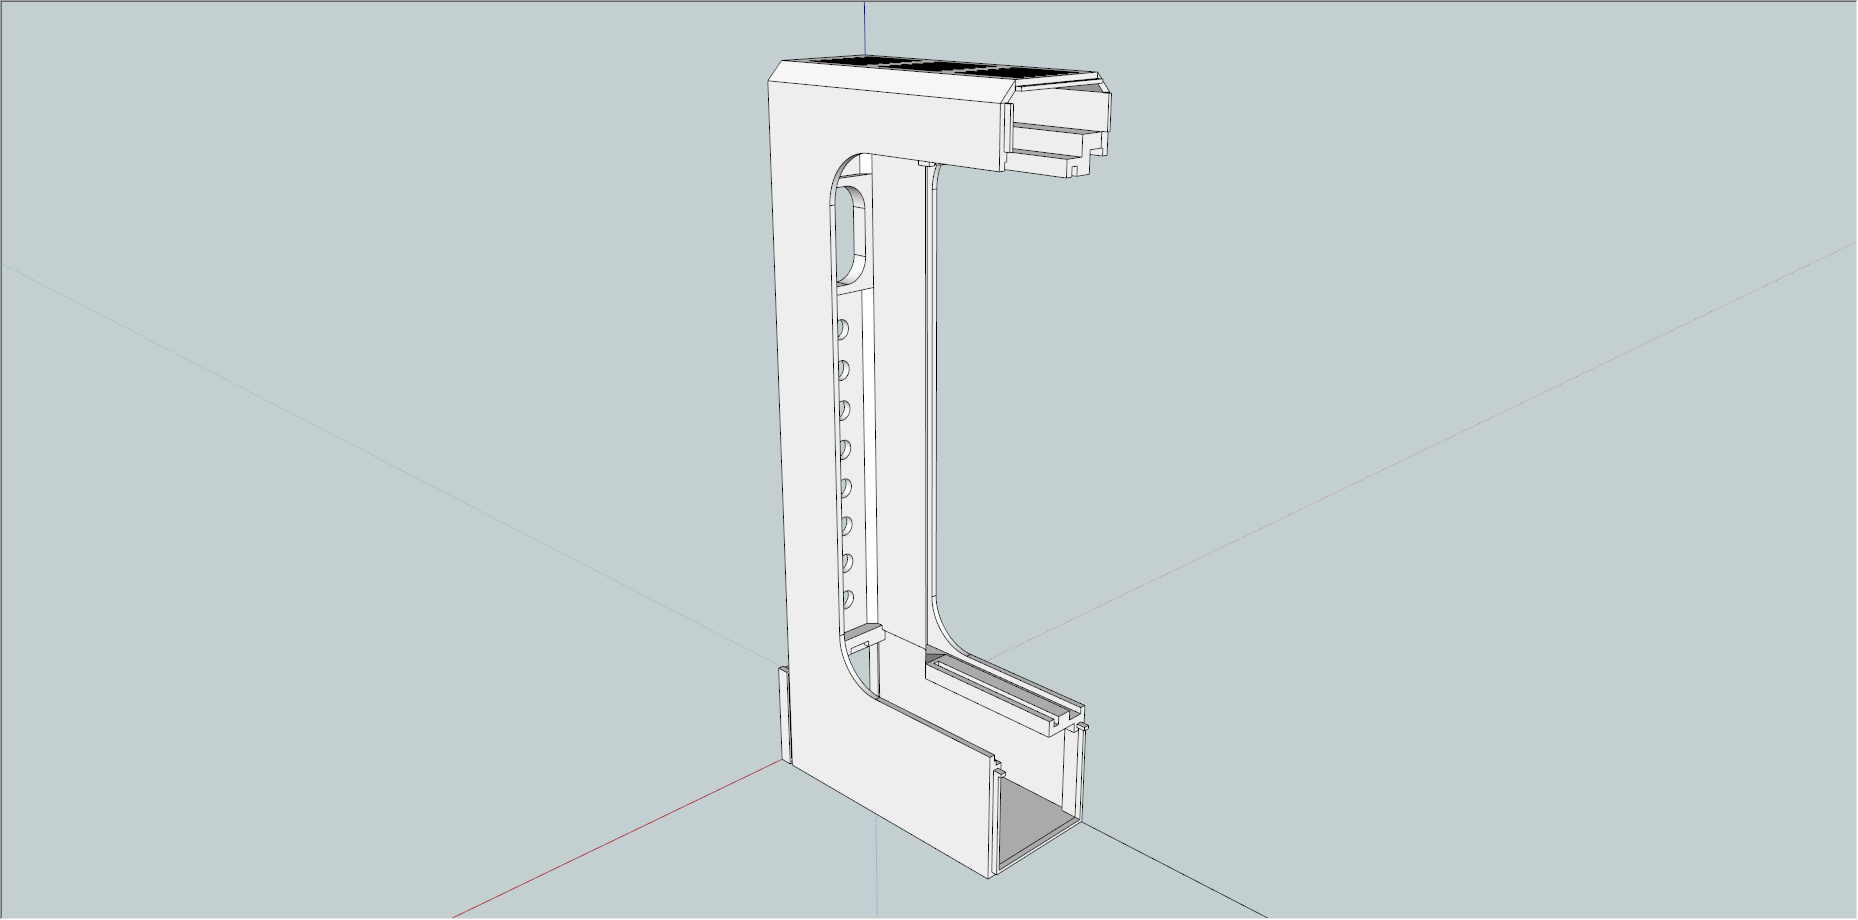
\includegraphics[width=\textwidth,keepaspectratio,clip]{appendix/screen-shots/case-front.png}%
\caption{The front of the case}
\end{figure}
\newpage
\begin{figure}
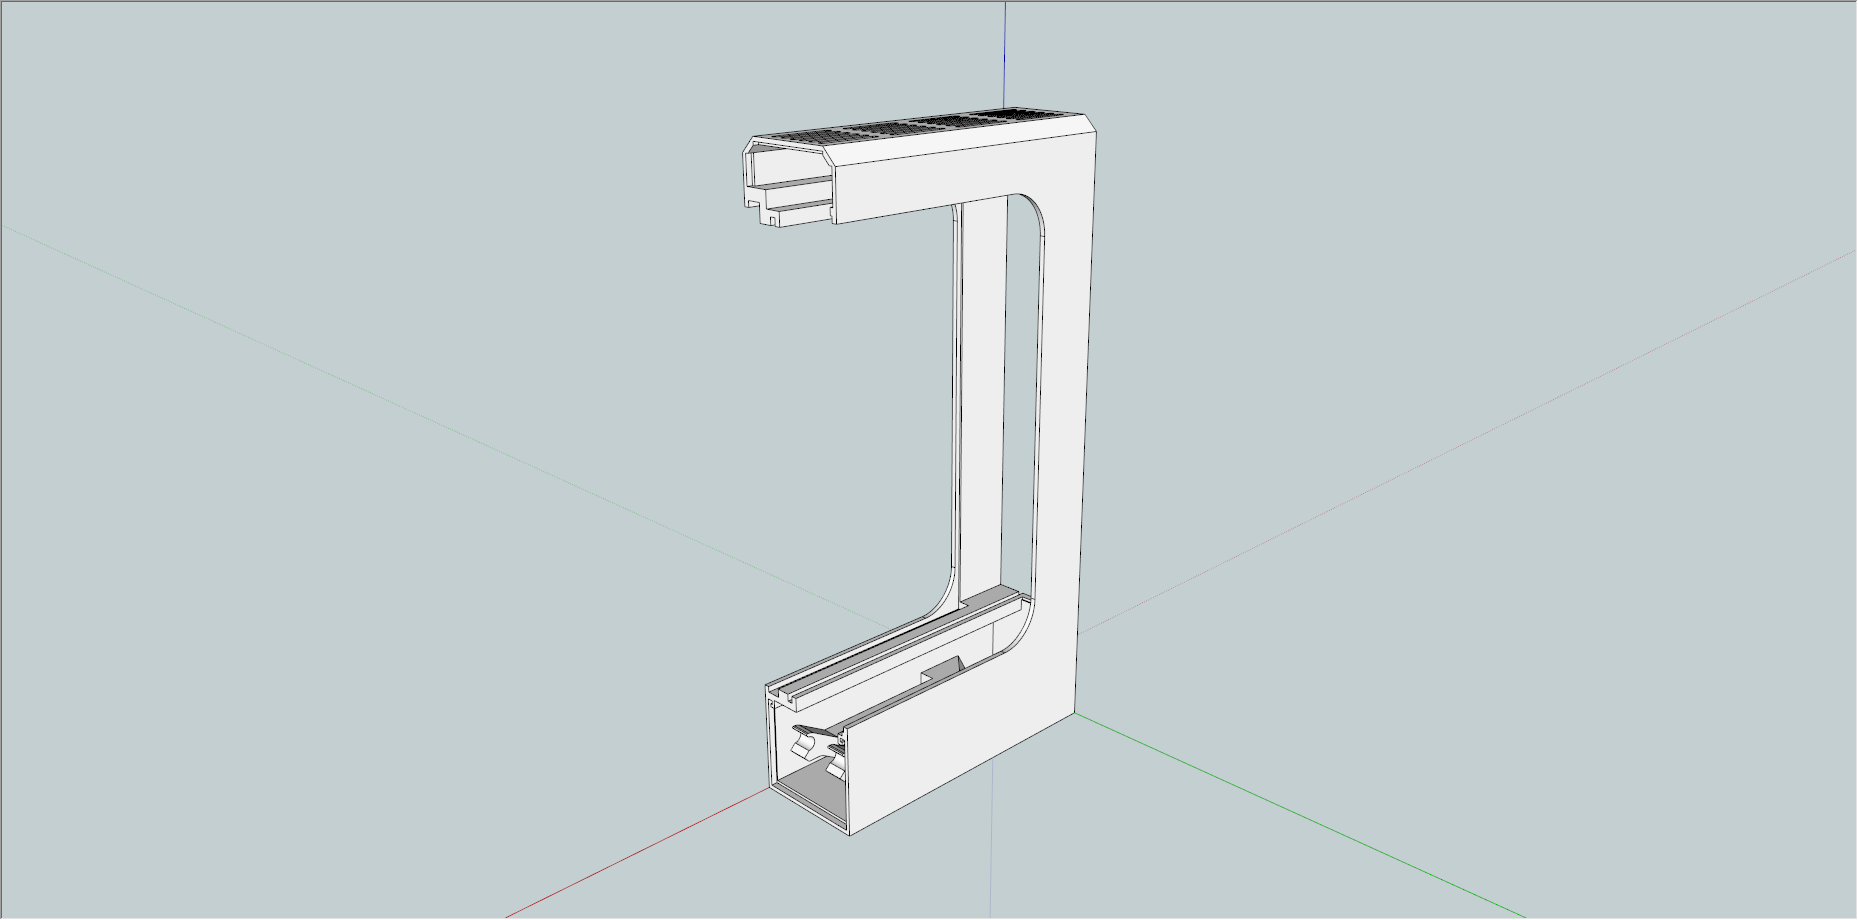
\includegraphics[width=\textwidth,keepaspectratio,clip]{appendix/screen-shots/case-back.png}%
\caption{The back of the case}
\end{figure}
\newpage
\begin{figure}
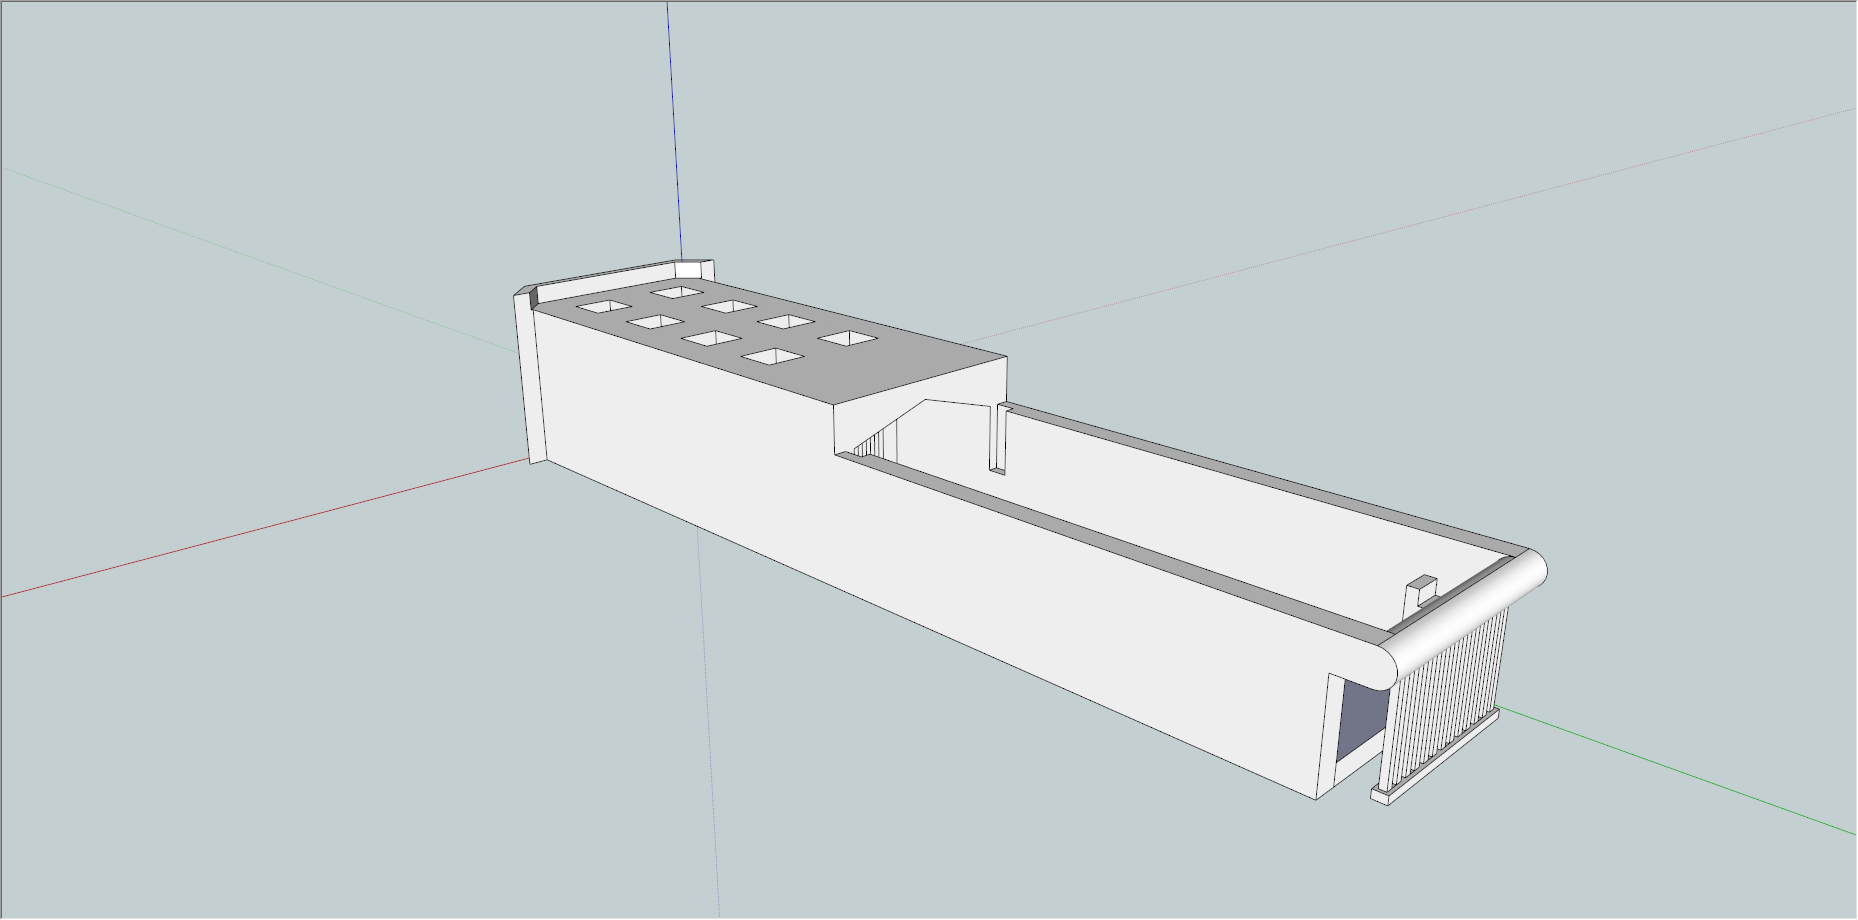
\includegraphics[width=\textwidth,keepaspectratio,clip]{appendix/screen-shots/keyboard.png}%
\caption{The keyboard tray}
\end{figure}
\newpage
\begin{figure}
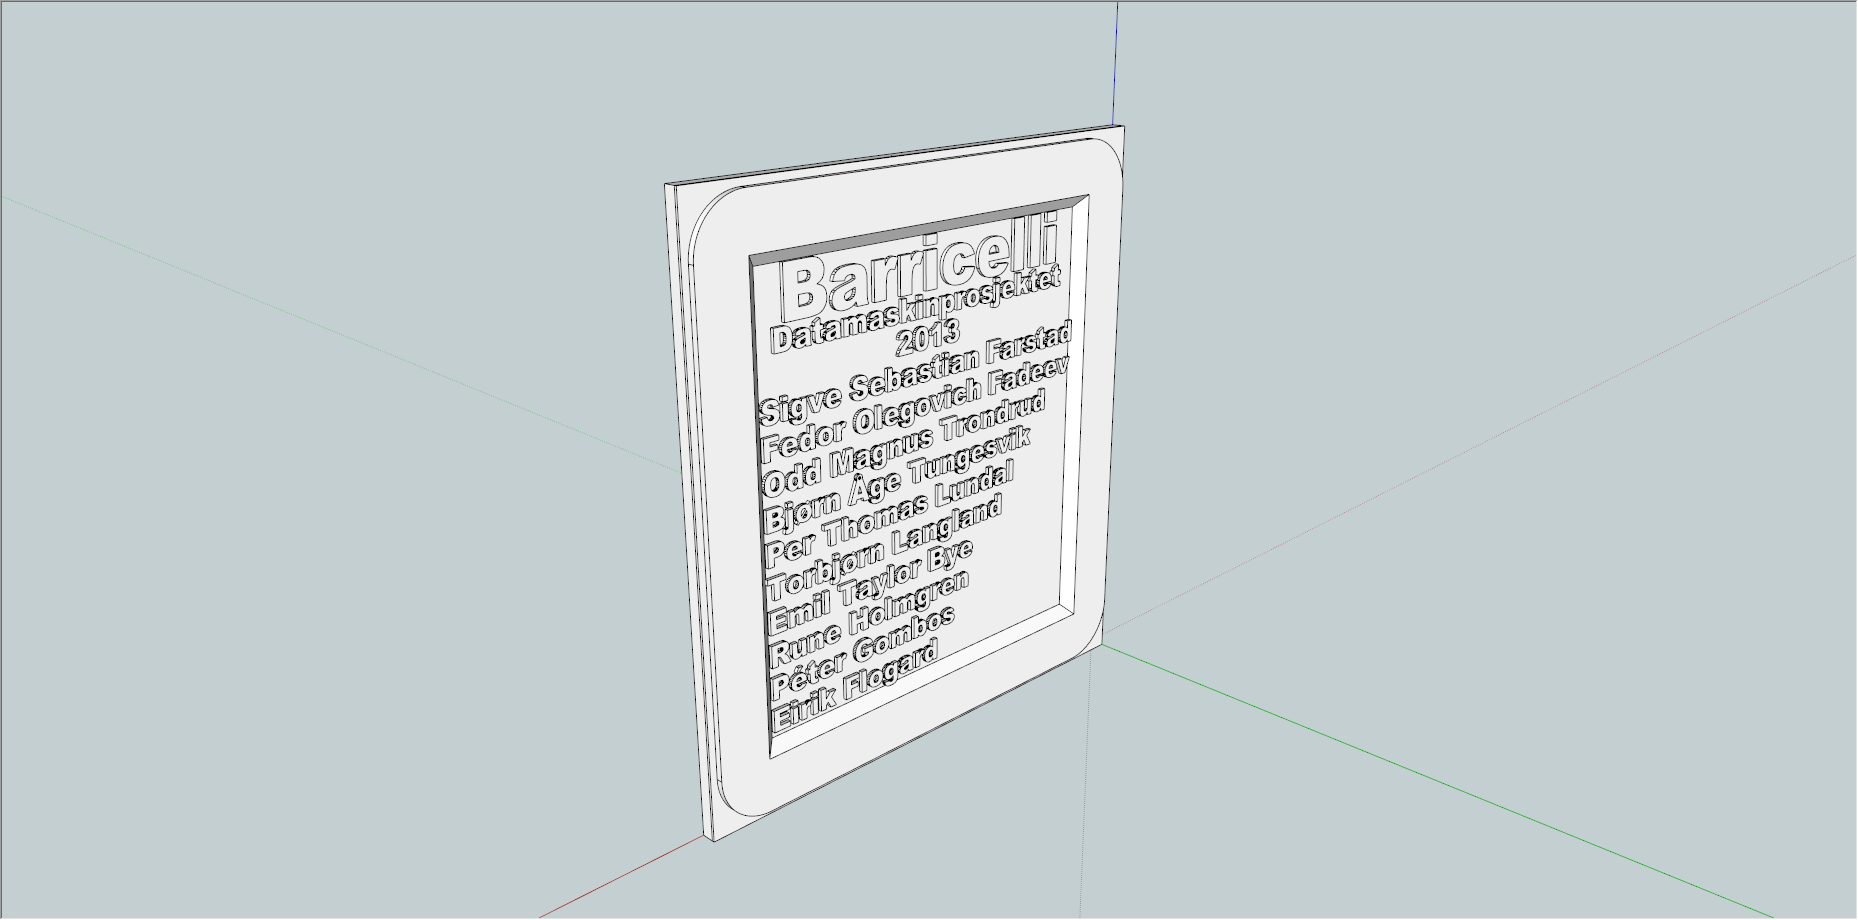
\includegraphics[width=\textwidth,keepaspectratio,clip]{appendix/screen-shots/names-side-panel.png}%
\caption{Side panel with the names of the team members}
\end{figure}
\newpage
\begin{figure}
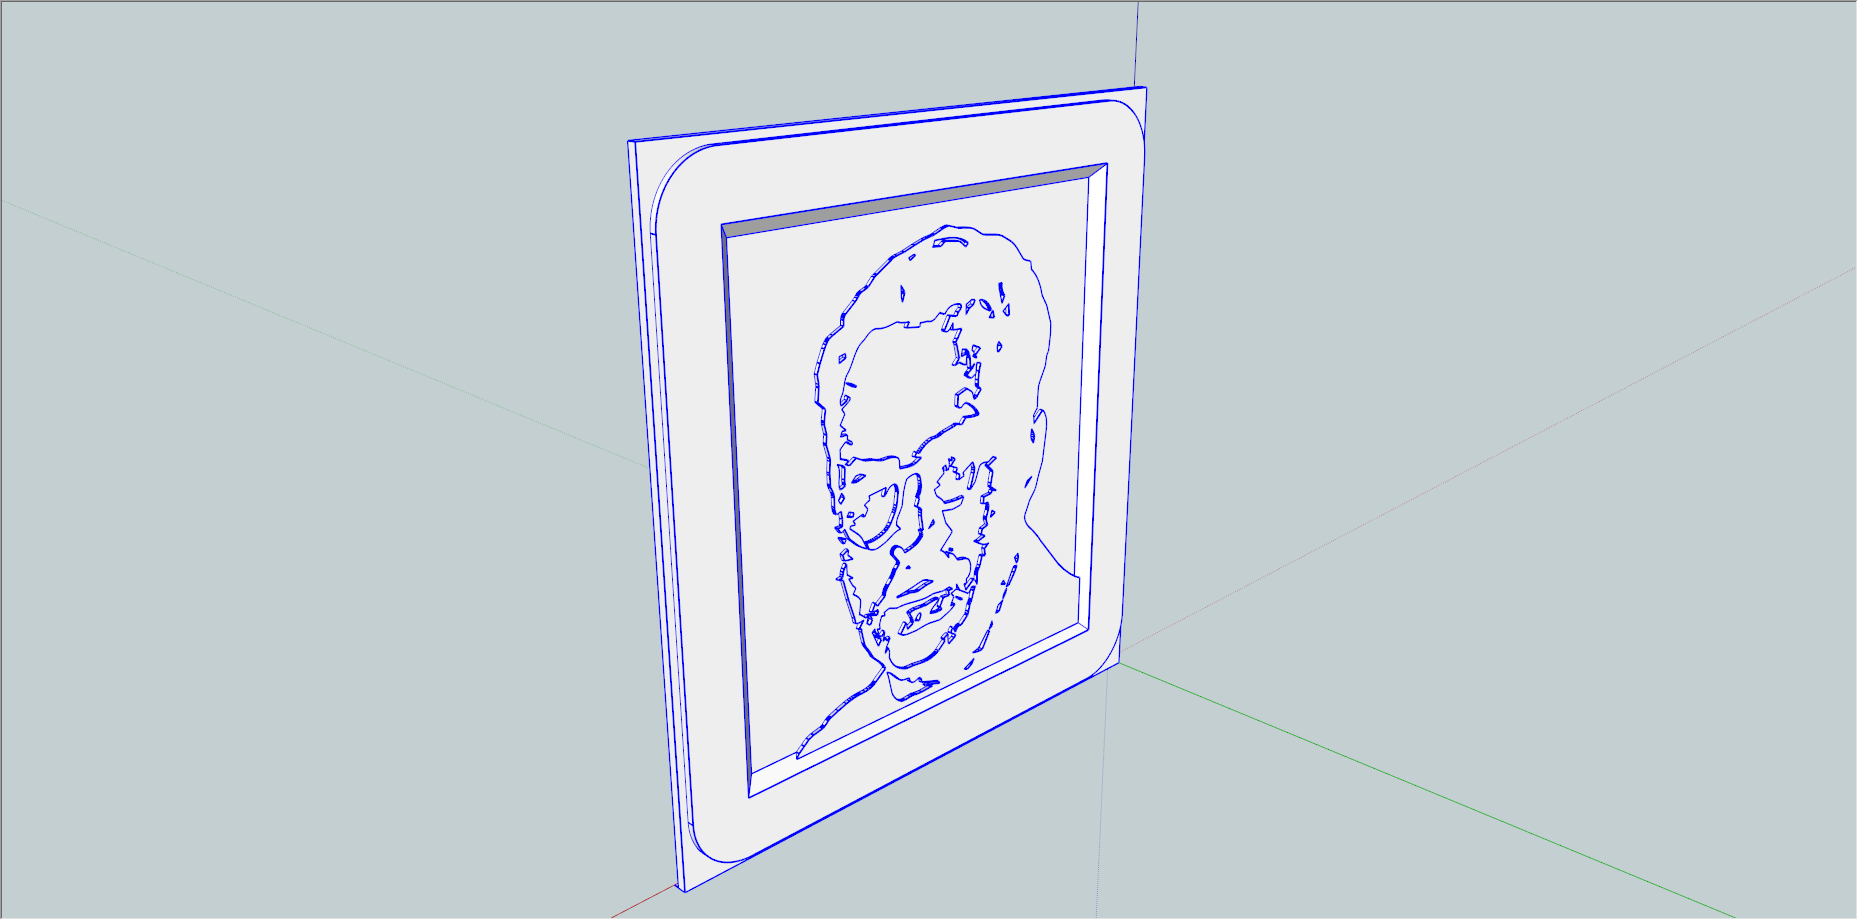
\includegraphics[width=\textwidth,keepaspectratio,clip]{appendix/screen-shots/barricelli-panel.png}%
\caption{The side panel with the picture of Nils Aall Barricelli}
\end{figure}
\newpage
\begin{figure}
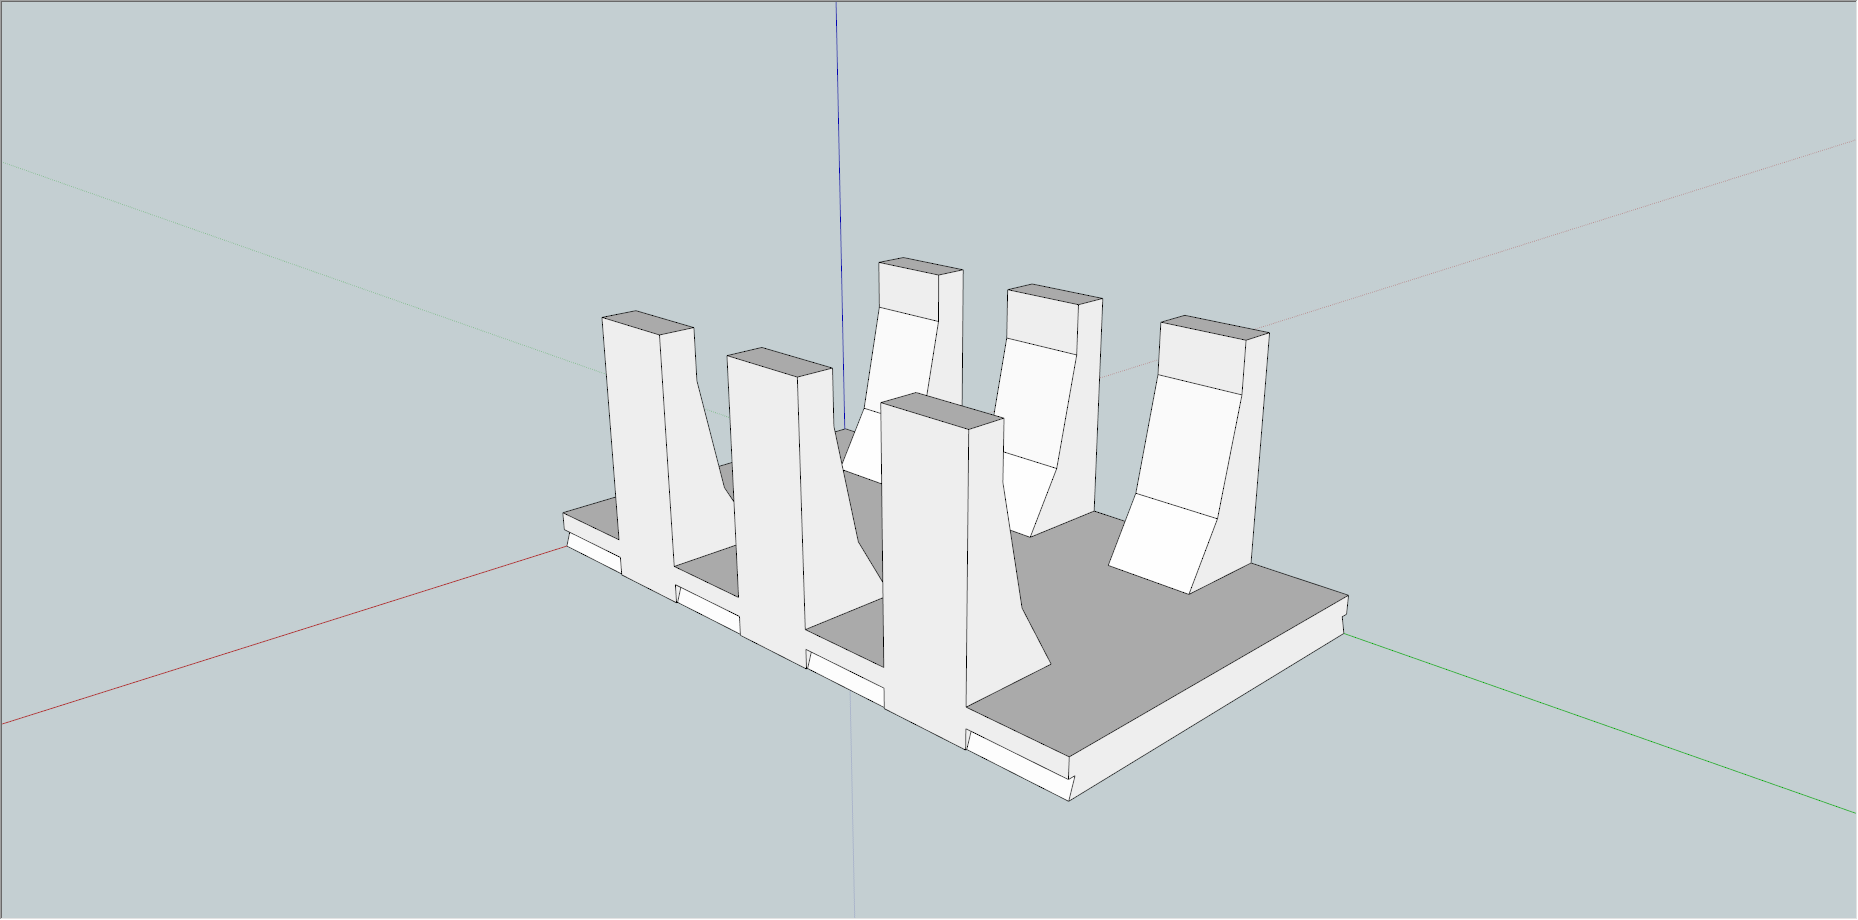
\includegraphics[width=\textwidth,keepaspectratio,clip]{appendix/screen-shots/keyboard-support.png}%
\caption{The support holding the buttons of the keyboard in place}
\end{figure}
\newpage
\begin{figure}
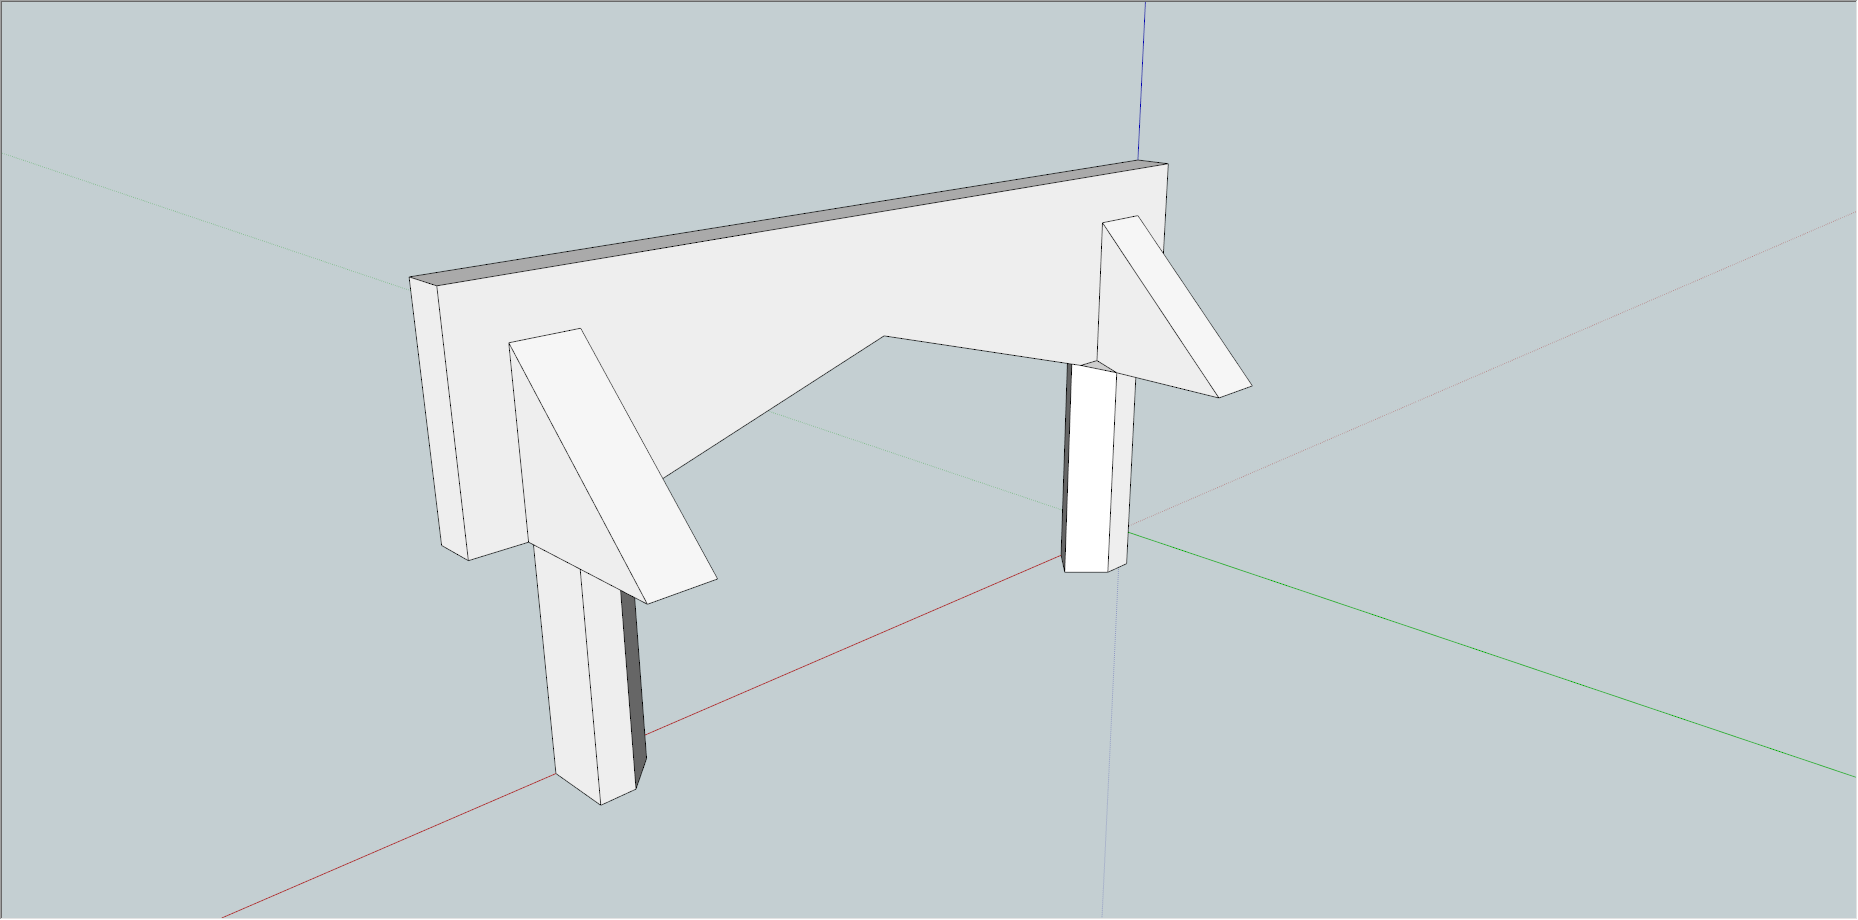
\includegraphics[width=\textwidth,keepaspectratio,clip]{appendix/screen-shots/keyboard-stopper.png}%
\caption{The plastic edge that stop the keyboard from sliding all the way out}
\end{figure}
\newpage
\begin{figure}
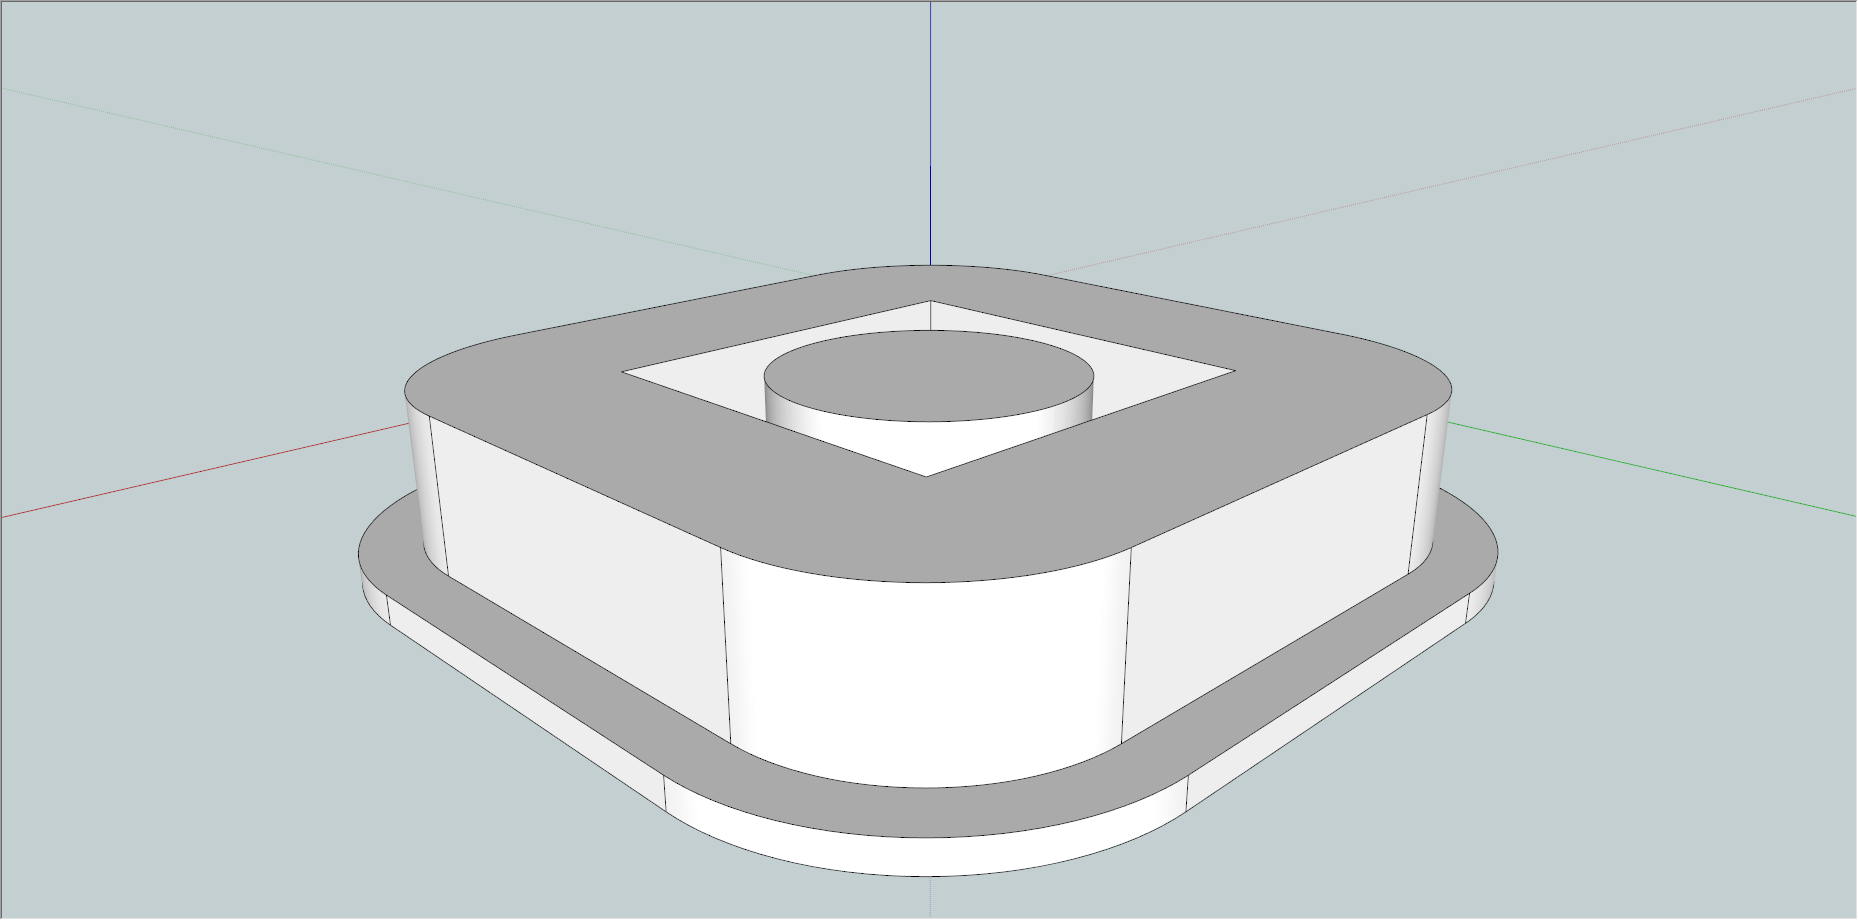
\includegraphics[width=\textwidth,keepaspectratio,clip]{appendix/screen-shots/ntnu-logo-blue.png}%
\caption{The blue part of the NTNU logo in front of the case}
\end{figure}
\newpage
\begin{figure}
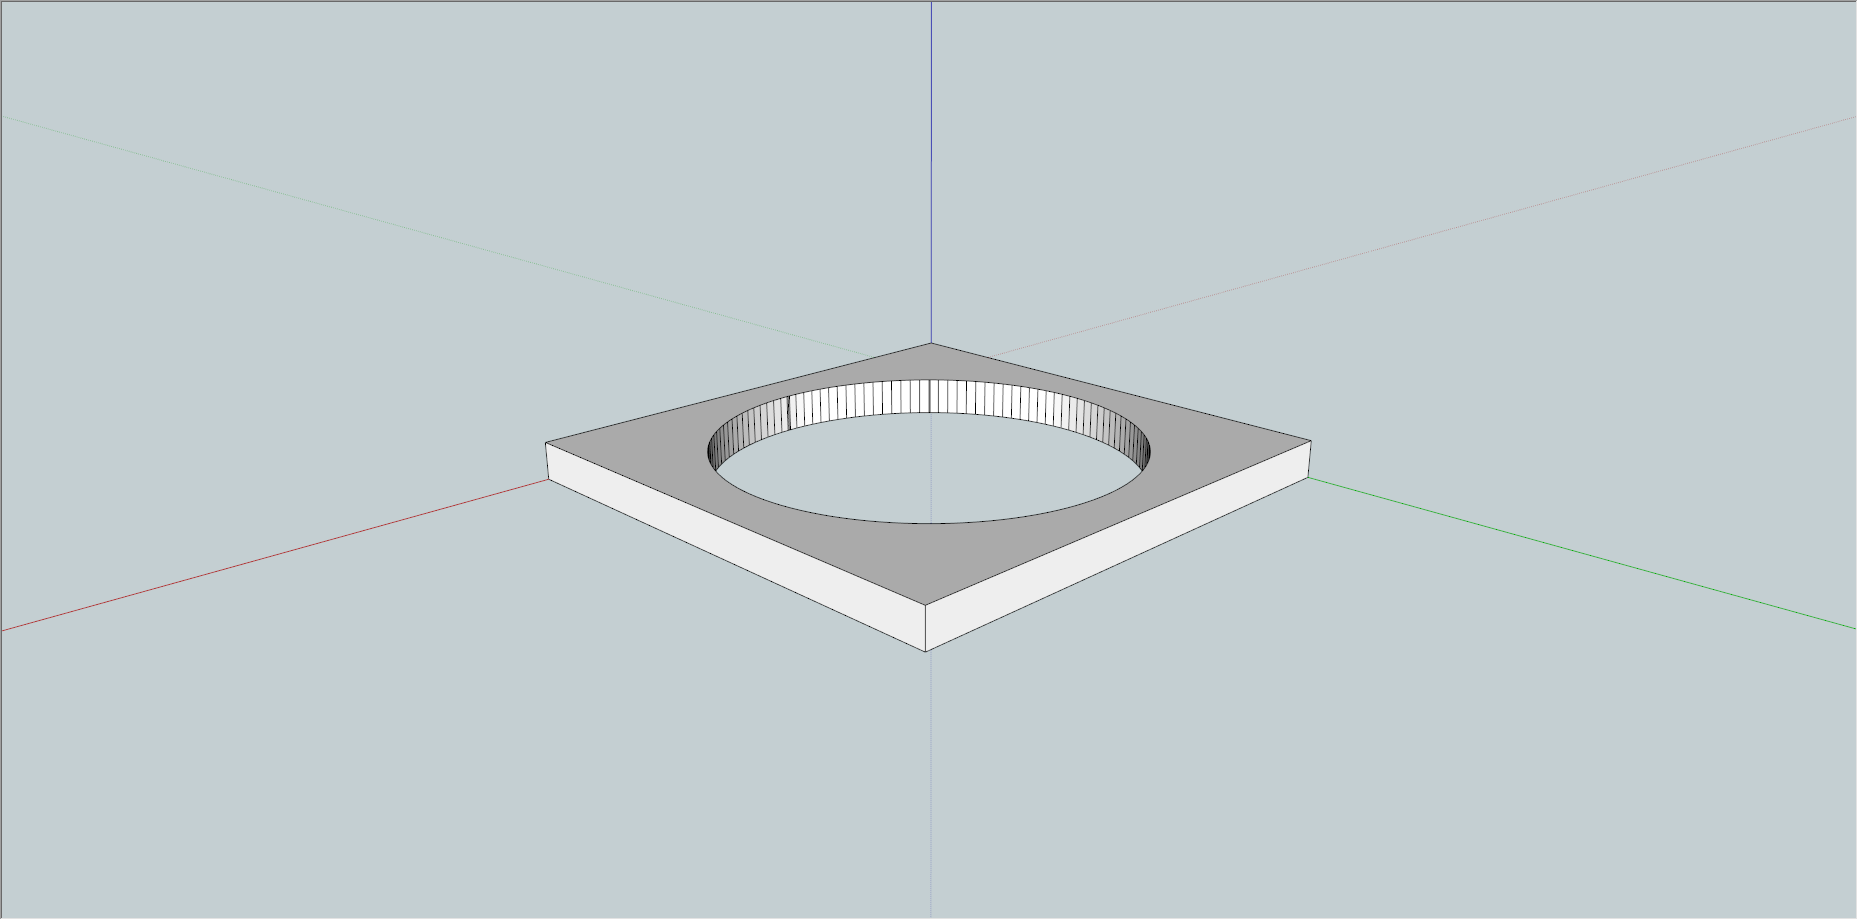
\includegraphics[width=\textwidth,keepaspectratio,clip]{appendix/screen-shots/ntnu-logo-yellow.png}%
\caption{The blue part of the NTNU logo in front of the case}
\end{figure}
\newpage
\begin{figure}
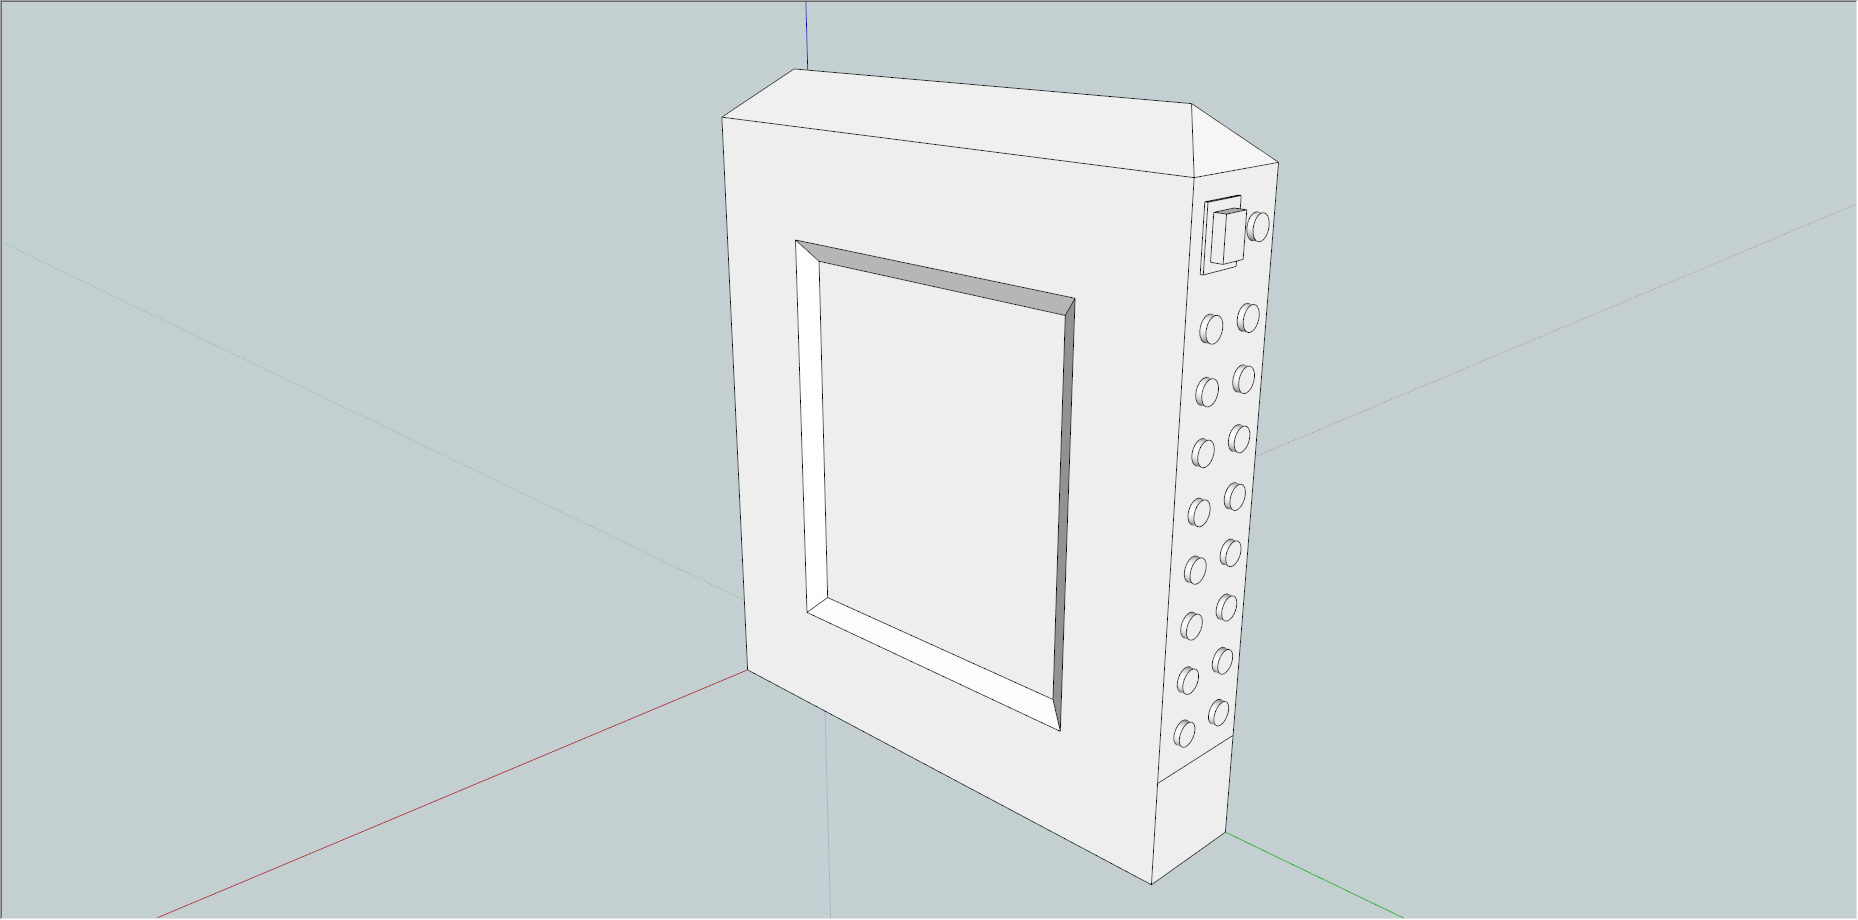
\includegraphics[width=\textwidth,keepaspectratio,clip]{appendix/screen-shots/early-case.png}%
\caption{An early sketch of the case}
\end{figure}

\chapter{Galapagos Assembler Listing} \label{appendix:galapagos-assembler-source-code}
\newpage

\lstinputlisting[language=Python]{galapagos-assembler/galapagos/__init__.py}
\lstinputlisting[language=Python]{galapagos-assembler/galapagos/assembler.py}
\lstinputlisting[language=Python]{galapagos-assembler/galapagos/base.py}
\lstinputlisting[language=Python]{galapagos-assembler/galapagos/instructions.py}
\lstinputlisting[language=Python]{galapagos-assembler/galapagos/scanner.py}

\chapter{Demonstration Program Listings} \label{appendix:demonstration-programs-source-code}
\newpage

\lstinputlisting[language={[x86masm]Assembler}]{GAS-programs/knapsack/solver.gas} \label{testing:listing:knapsack}
\lstinputlisting[language={[x86masm]Assembler}]{GAS-programs/simple_memtest/memtest.gas}
\lstinputlisting[language={[x86masm]Assembler}]{GAS-programs/color-search/color-search.gas} \label{testing:listing:color-search}

\chapter{Test Bench Documentation} \label{appendix:test-bench-documentation}
\newpage

\section{Introduction}
This document provides additional documentation and graphics from unit test benches, used for verifying the components in the FPGA.
The graphics are selected screenshots taken in ISim.  

\section{Component Tests}

\subsection{Fitness Core}
In order to test the fitness cores a set of small assembly programs were created. These programs aims to test various cases in the galapagos architecture. The tests are included here for reference.

\paragraph{RRR-RRI Instructions}
Simple program testing the use of RRI and RRR instructions


\lstinputlisting[language={[x86masm]Assembler}]{testing/gas-listings/rrr-rri.gas}\label{testing:listing:rrr-rri}


\paragraph{Store instruction}
Demonstrating the store instruction

\lstinputlisting[language={[x86masm]Assembler}]{testing/gas-listings/store.gas}\label{testing:listing:store}

\paragraph{Load instruction}
Demonstrating the load instruction instruction

\lstinputlisting[language={[x86masm]Assembler}]{testing/gas-listings/load.gas}\label{testing:listing:load}

\paragraph{Conditional execute}
Demonstrating code with conditionals that evaluate to true. 

\lstinputlisting[language={[x86masm]Assembler}]{testing/gas-listings/conditional-executed.gas}\label{testing:listing:conditional-executed}

\paragraph{Conditional non-execute}
Demonstrating code with conditionals that evaluate to false. 

\lstinputlisting[language={[x86masm]Assembler}]{testing/gas-listings/conditional-not-executed.gas}\label{testing:listing:conditional-not-executed}

\paragraph{Branch taken}
Demonstrating an conditional branch where the conditional is evaluated to true.  

\lstinputlisting[language={[x86masm]Assembler}]{testing/gas-listings/branch-taken.gas}\label{testing:listing:branch-taken}

\paragraph{Branch not-taken}
Demonstrating an conditional branch where the conditional is evaluated to false.  

\lstinputlisting[language={[x86masm]Assembler}]{testing/gas-listings/branch-not-taken.gas}\label{testing:listing:branch-not-taken}

\paragraph{Store gene}
Demonstrate the use of the store gene instruction. 

\lstinputlisting[language={[x86masm]Assembler}]{testing/gas-listings/store-gene.gas}\label{testing:listing:store-gene}

\paragraph{Load gene}
Demonstrate the use of the load gene instruction. 
\lstinputlisting[language={[x86masm]Assembler}]{testing/gas-listings/load-gene.gas}\label{testing:listing:load-gene}




\subsection{Genetic Pipeline}

\subsubsection{Selection Core}
\subsubsection{Crossover Core} 
\begin{figure}[H]
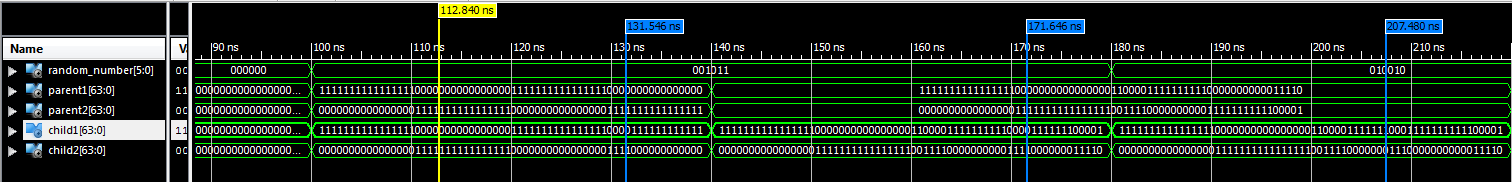
\includegraphics[width=\textwidth]{fpga/fig/testbenches/crossover_split_simulation1.png}
\caption{Crossover Split Simulation Screenshot}
\label{fig_crossover_split_testbench}
\end{figure}

Figure \ref{fig_crossover_split_testbench} shows the simulation of Crossover Split function, where the blue markers are set just before the crossover begins. 
Changes in input parents and random\_number causes changes in children. 

\begin{figure}[H]
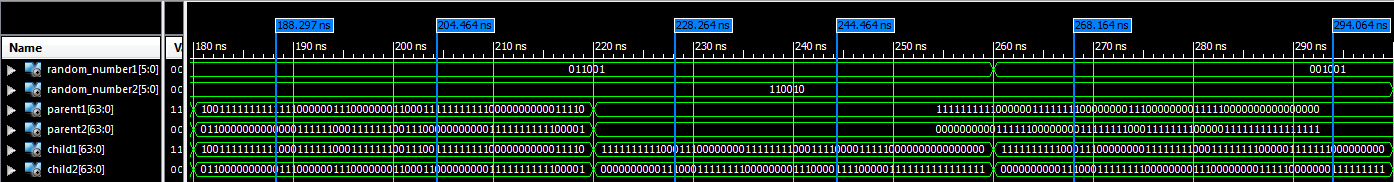
\includegraphics[width=\textwidth]{fpga/fig/testbenches/crossover_doublesplit_simulation1.png}
\caption{Crossover Double-Split Simulation Screenshot}
\label{fig_crossover_doublesplit_testbench}
\end{figure}

Figure \ref{fig_crossover_doublesplit_testbench} shows the simulation of Crossover Double-Split function, where the blue markers are set alternating before and after crossover.
Changes in input parents and any random\_number causes changes in children. 

\begin{figure}[H]
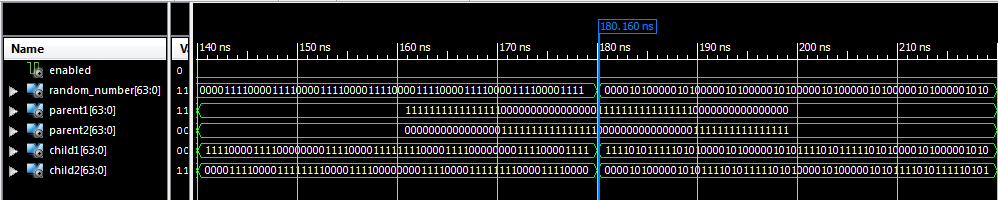
\includegraphics[width=\textwidth]{fpga/fig/testbenches/crossover_xor_simulation1.png}
\caption{Crossover XOR Simulation Screenshot}
\label{fig_crossover_xor_testbench}
\end{figure}

Figure \ref{fig_crossover_xor_testbench} shows the simulation of Crossover XOR function, where the blue marker is set at a change in the random\_number, causing changes on the crossover in the children.
Changes in input parents and any random\_number causes changes in children. 

\begin{figure}[H]
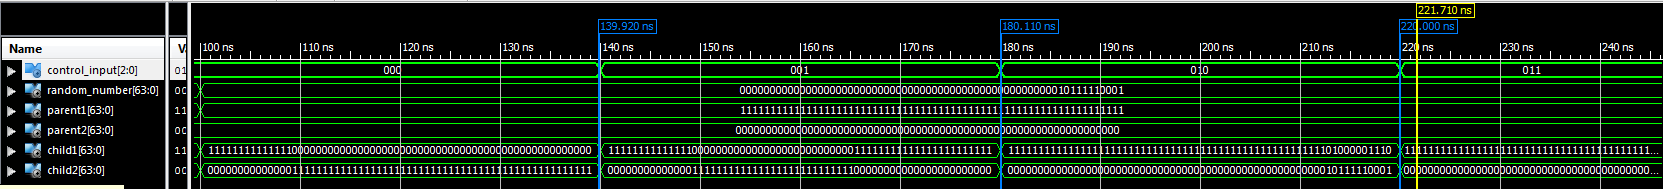
\includegraphics[width=\textwidth]{fpga/fig/testbenches/crossover_toplevel_testbench.png}
\caption{Crossover Toplevel Simulation Screenshot}
\label{fig_crossover_toplevel_testbench}
\end{figure}

Figure \ref{fig_crossover_toplevel_testbench} shows the simulation of Crossover toplevel, where the blue markers are set at changes in the control\_input, changing from split to double-split, then to XOR, and finally to no crossover at all.

\subsubsection{Mutation Core}
\begin{figure}[H]
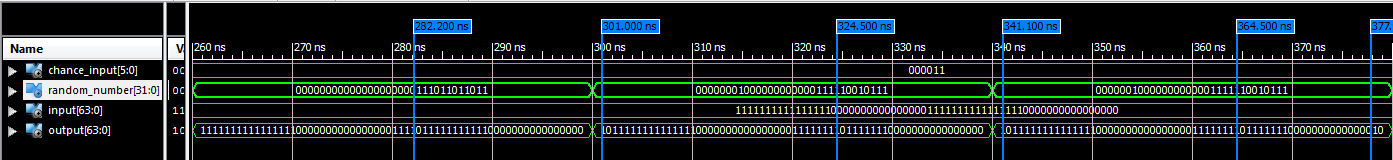
\includegraphics[width=\textwidth]{fpga/fig/testbenches/mutation_simulation1.png}
\caption{Mutation Core Simulation Screenshot 1}
\label{fig_mutation_testbench1}
\end{figure}

Figure \ref{fig_mutation_testbench1} shows the simulation of the Mutation Core, where the blue markers are set just before the bits that are mutated in the output.
Figure \ref{fig_mutation_testbench2} shows another part of the same simulation, with different main input.

\begin{figure}[H]
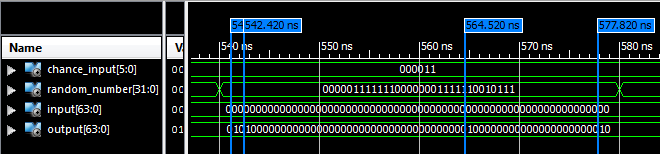
\includegraphics[width=\textwidth]{fpga/fig/testbenches/mutation_simulation2.png}
\caption{Mutation Core Simulation Screenshot 2}
\label{fig_mutation_testbench2}
\end{figure}


\chapter{PCB Components} \label{appendix:components}
This is the list of components used in the production of Barricelli.

With the exception of the FPGA and Microcontroller, all components were ordered from Farnell and are listed with their farnell product number.
The FPGA and microcontroller were ordered from Digi-Key and are listed with their full identifiers instead.

\begin{table}[H]
\begin{center}
\begin{tabular}{| l | r | r|}
\hline
\textbf{Component} & \textbf{Farnell product \textnumero} & \textbf{\textnumero required} \\
\hline
Oscillator  & 1842148 & 1 \\
\hline
Jumpers  & 4218176 & 86 \\
\hline
Headers  & 1580053 & 278 \\
\hline
EFM32GG390F1024-BGA112 & Ordered from digi-key & 1 \\
\hline
XC6SLX45-2CSG324I & Ordered from digi-key & 1 \\
\hline
Serial Port Connector  & 1653978 & 1 \\
\hline
Serial Port Driver  & 1287435 & 1 \\
\hline
Power Connector  & 224960 & 1 \\
\hline
Memory Chip  & 2103743 & 3 \\
\hline
LED, red  & 8554510 & 6 \\
\hline
LED, green  & 5790852 & 16 \\
\hline
micro USB Receptacle  & 2293751 & 1 \\
\hline
SD Card Receptacle  & 2226409 & 1 \\
\hline
Voltage Regulator  & 1685484 & 1 \\
\hline
Voltage Regulator 3.3V  & 1469037 & 1 \\
\hline
Switch (button)  & 3801287 & 8 \\
\hline
Switch (toggle)  & 1524244 & 1 \\
\hline
Transient Voltage Suppressor  & 1748616 & 1 \\
\hline
ESD Suppressor (30V VCL)  & 1850152 & 1 \\
\hline
ESD Suppressor (17V VCL)  & 1850151 & 1 \\
\hline
Resistor 50k R & 2057780 & 7 \\
\hline
Resistor 0 R & 1653183 & 1 \\
\hline
Resistor 56 R & 1738995 & 18 \\
\hline
Resistor 105 R & 2139353 & 1 \\
\hline
Resistor 120 R & 1470033 & 1 \\
\hline
Resistor 330 R & 2333547 & 3 \\
\hline
Resistor 100k R & 9240764 & 1 \\
\hline
Capacitor 100 nF & 1759297 & 59 \\
\hline
Capacitor 1 uF & 1759455 & 3 \\
\hline
Capacitor 4.7 uF & 1759444 & 1 \\
\hline
Capacitor (Electrolyte) 100 nF & 9697039 & 5 \\
\hline
Capacitor (Electrolyte) 10 uF & 2326109 & 4 \\
\hline
\end{tabular}
\end{center}
\end{table}

\newpage
